\subsection{外代数的反交换性}

命题5. (i) 设 \((x_{i})_{1\leqslant i\leqslant n}\) 为模 \(\mathbf{M}\) 的元素组成的有限序列；对于每个置换 \(\sigma\) （对称群 \(\mathfrak{S}_n\) 中的），

\[
x _ {\sigma (1)} \wedge x _ {\sigma (2)} \wedge \dots \wedge x _ {\sigma (n)} = \varepsilon_ {\sigma}. x _ {1} \wedge x _ {2} \wedge \dots \wedge x _ {n}\tag{6}
\]

其中 \(\varepsilon_{\sigma}\) 表示置换 \(\sigma\) 的符号。

\begin{enumerate}
\def\labelenumi{(\roman{enumi})}
\setcounter{enumi}{1}
\tightlist
\item
  如果存在两个不同的指标 \(i, j\) 使得 \(x_{i} = x_{j}\) ，则乘积
\end{enumerate}

\[
x _ {1} \wedge x _ {2} \wedge \dots \wedge x _ {n}
\]

为零。

\begin{enumerate}
\def\labelenumi{(\roman{enumi})}
\tightlist
\item
  首先，由于 \(x \wedge x = 0\) 对所有 \(x \in \mathbf{M}\) 成立（由理想 \(\mathfrak{J}''\) 的定义可知），此外，对于 \(x, y\) 属于 \(\mathbf{M}\) 的情形，
\end{enumerate}

\[
x \wedge y + y \wedge x = (x + y) \wedge (x + y) - x \wedge x - y \wedge y = 0.
\]

这确立了（6）在 \(n = 2\) 的情形。一般情形随后由 §4 第 6 号的引理 3 得出。

\begin{enumerate}
\def\labelenumi{(\roman{enumi})}
\setcounter{enumi}{1}
\tightlist
\item
  在 (ii) 的假设下，存在一个置换 \(\sigma \in \mathfrak{S}_n\) ，使得 \(\sigma(1) = i\) 和 \(\sigma(2) = j\) ；那么对这个置换而言，(6) 的左边为零，因此右边也为零。
\end{enumerate}

推论 1. 设 H, K 为 N 的区间 \([1, n]\) 的两个互补子集，并设 \((i_{h})_{1 \leqslant h \leqslant p}, (j_{k})_{1 \leqslant k \leqslant n - p}\) 分别按递增顺序排列的 H 和 K 的元素序列；我们记

\[
x _ {H} = x _ {i _ {1}} \wedge x _ {i _ {2}} \wedge \dots \wedge x _ {i _ {p}}, \quad x _ {K} = x _ {j _ {1}} \wedge x _ {j _ {2}} \wedge \dots \wedge x _ {j _ {n - p}};
\]

那么

\[
x _ {\mathrm{H}} \wedge x _ {\mathrm{K}} = (- 1) ^ {\nu} x _ {1} \wedge x _ {2} \wedge \dots \wedge x _ {n}\tag{7}
\]

其中 \(\nu\) 是有序对 \((i,j)\in \mathbf{H}\times \mathbf{K}\) 中满足 \(i > j\) 者的个数

根据命题5，这归结为证明

引理 1. 若 \(\sigma \in \mathfrak{S}_n\) 是满足 \(\sigma(h) = i_h\) （对 \(1 \leqslant h \leqslant p\) ）与 \(\sigma(h) = j_{h-p}\) （对 \(p + 1 \leqslant h \leqslant n\) ）的置换，则 \(\varepsilon_\sigma = (-1)^{\nu}\) .

对于 \(1 \leqslant h < h' \leqslant p\) 或 \(p + 1 \leqslant h < h' \leqslant n\) ，有 \(\sigma(h') > \sigma(h)\) ，而有序对 \((h, h')\) ——即满足 \(1 \leqslant h \leqslant p < h' \leqslant n\) 与 \(\sigma(h) > \sigma(h')\) 者——的个数等于 \(\nu\) .

推论 2. 分次代数 \(\bigwedge (\mathbf{M})\) 是交错的（§ 4，第 9 号）。

只需将 §4 第 9 号的命题 13 应用于 \(\bigwedge (\mathbf{M})\) ，取生成系为集合 \(\mathbf{M}\) 并利用命题5。

命题6. 若 M 是有限生成的 A-模，则 \(\bigwedge (\mathbf{M})\) 是有限生成的 A-模；此外，若 M 具有含 \(n\) 个元素的生成系，则 \(\bigwedge^{p}(\mathbf{M}) = \{0\}\) 对于 \(p > n\) .

设 \((x_{i})_{1\leqslant i\leqslant n}\) 为 M 的一个生成系。\(\bigwedge^{p}(\mathbf{M})\) 中的每个元素都是形如

\[
x _ {i _ {1}} \wedge x _ {i _ {2}} \wedge \dots \wedge x _ {i _ {p}}
\]

其中指标 \(i_k\) 属于 \([1, n]\) ；根据命题 5，可设这些指标互不相同（否则相应的元素为零）。如果 \(p > n\) ，则不存在这样的指标序列，因此 \(\bigwedge^p(\mathbf{M}) = \{0\}\) 。若 \(p \leqslant n\) ，这样的序列只有有限多个，这就完成了证明。

\subsection{模的n次外幂与交错多重线性映射}

给定交换环 A 上的两个模 M、N，从 \(M^{n}\) 到 N 的交错 n-线性映射是指这样的 n-线性映射 \(f: M^{n} \to N\) ：对所有 \(p \leqslant n - 2\) ，

\[
f (u _ {1}, \dots , u _ {p}, x, x, v _ {1}, \dots , v _ {n - p - 2}) = 0\tag{8}
\]

对所有 \(x\) ，所有 \(u_{i}\) ( \(1 \leqslant i \leqslant p\) ) 以及所有 \(v_{j}\) ( \(1 \leqslant j \leqslant n - p - 2\) ) 在 \(\mathbf{M}\) 中均成立。

命题7. 设 A 为交换环，M 和 N 为两个 A-模。若对每个 A-线性映射 \(g: \bigwedge^n (\mathbf{M}) \to \mathbf{N} (n \geqslant 2)\) 使之对应于 n-线性映射

\[
\left(x _ {1}, x _ {2}, \dots , x _ {n}\right) \mapsto g \left(x _ {1} \wedge x _ {2} \wedge \dots \wedge x _ {n}\right)\tag{9}
\]

便得到从 A-模 \(\operatorname{Hom}_{\mathbf{A}}(\bigwedge^{n}(\mathbf{M}), \mathbf{N})\) 到由交错 \(n\) -线性映射（从 \(\mathbf{M}^n\) 到 \(\mathbf{N}\) 的）所组成的 A-模上的一个双射 A-线性映射。

我们考虑 A-模 \(\operatorname{Hom}_{\mathbf{A}}(\mathsf{T}^{n}(\mathbf{M}),\mathbf{N})\) 到 A-模 \(\mathcal{L}_{n}(\mathbf{M},\ldots,\mathbf{M};\mathbf{N})\) （即所有从 \(M^{n}\) 到 N 的 n-线性映射组成的 A-模）的典范双射，它通过将每个 A-线性映射 \(f: T^{n}(\mathbf{M}) \to \mathbf{N}\) 对应于 n-线性映射而得到

\[
\bar {f} \colon (x _ {1}, \dots , x _ {n}) \mapsto f (x _ {1} \otimes x _ {2} \otimes \dots \otimes x _ {n})
\]

(II, § 3, no. 9)。另一方面，A-线性映射 \(g \colon \bigwedge^{n}(\mathbf{M}) \to \mathbf{N}\) 与 A-线性映射 \(f \colon \mathsf{T}^n (\mathbf{M}) \to \mathbf{N}\) （满足 \(f\) 在 \(\mathfrak{J}_n''\) 上为零者）一一对应，其对应方式是把 \(g\) 映为 \(f = g \circ p_n\) ，其中

\[
p _ {n} \colon \mathsf {T} ^ {n} (\mathbf {M}) \rightarrow \bigwedge^ {n} (\mathbf {M}) = \mathsf {T} ^ {n} (\mathbf {M}) / \mathfrak {J} _ {n} ^ {\prime \prime}
\]

是典范同态（II，§2，第 1 号，定理 1）。但鉴于 \(\mathfrak{J}_n''\) 是形如

\[
\left(u _ {1} \otimes u _ {2} \otimes \dots \otimes u _ {p}\right) \otimes (x \otimes x) \otimes \left(v _ {1} \otimes \dots \otimes v _ {n - p - 2}\right)
\]

\((x, u_{i}, v_{j} \text{ 属于 M}), \text{ 说 } f \text{ 具有形式 } g \circ p_{n} \text{ 意味着相应的 } n\text{-线性函数 } \bar{f} \text{ 满足 (8)，换言之它是交错的。}\)

A-模 \(\bigwedge^{n}(\mathbf{M})\) 称为 \(n\) -次外幂（即 \(\mathbf{M}\) 的外幂）。对于每个 A-模同态 \(u: \mathbf{M} \to \mathbf{N}\) ，映射

\[
\bigwedge^ {n} (u): \bigwedge^ {n} (\mathbf {M}) \rightarrow \bigwedge^ {n} (\mathbf {N})
\]

它与 \(\bigwedge(u)\) 在 \(\bigwedge^{n}(\mathbf{M})\) 上的限制相一致，称为 \(n\) -次外幂（即 \(u\) 的外幂）.

推论 1. 对于每个交错 \(n\) -线性映射 \(g: \mathbf{M}^n \to \mathbf{N}\) ，对于每个置换 \(\sigma \in \mathfrak{S}_n\) ,

\[
g \left(x _ {\sigma (1)}, x _ {\sigma (2)}, \dots , x _ {\sigma (n)}\right) = \varepsilon_ {\sigma}. g \left(x _ {1}, x _ {2}, \dots , x _ {n}\right)\tag{10}
\]

对所有 \(x_{i} \in \mathbf{M}\) 成立；此外，若 \(x_{i} = x_{j}\) 对于两个不同的指标 \(i, j\) 成立，则

\[
g (x _ {1}, x _ {2}, \dots , x _ {n}) = 0.
\]

这是命题 7 以及第 3 号命题 5 的明显推论。

推论2. 设 \((x_{i})_{1\leqslant i\leqslant n}\) 是由 \(n\) 个元素组成的一个序列（元素属于 \(\mathbf{M}\) ），使得

\[
x _ {1} \wedge x _ {2} \wedge \dots \wedge x _ {n} = 0;
\]

那么，对于每一个交错的 \(n\) -线性映射 \(g: \mathbf{M}^n \to \mathbf{N}\) , \(g(x_1, \ldots, x_n) = 0\) .

推论3. 设 \(f: \mathbf{M}^{n-1} \to \mathbf{A}\) 是一个交错 \((n-1)\) -线性形式。如果 \((x_i)_{1 \leq i \leq n}\) 是由 \(n\) 个元素组成的一个序列（元素属于 \(\mathbf{M}\) ），使得 \(x_1 \wedge x_2 \wedge \cdots \wedge x_n = 0\) ，则

\[
\sum_ {i = 1} ^ {n} (- 1) ^ {i} f (x _ {1}, \dots , \hat {x _ {i}}, \dots , x _ {n}). x _ {i} = 0\tag{11}
\]

（其中我们记 \(f(x_{1},\ldots ,\hat{x}_{i},\ldots ,x_{n}) = f(x_{1},\ldots ,x_{i - 1},x_{i + 1},\ldots ,x_{n})\) 对于 \(1\leqslant i\leqslant n\) .

只需证明这个 n-线性映射

\[
(x _ {1}, \dots , x _ {n}) \mapsto \sum_ {i = 1} ^ {n} (- 1) ^ {i} f (x _ {1}, \dots , \hat {x} _ {i}, \dots , x _ {n}). x _ {i}
\]

从 \(M^{n}\) 到 M 是交错的。现在，若 \(x_{i} = x_{i+1}\) ，则由于 f 是交错的，右端求和中除 \(x_{i}\) 与 \(x_{i+1}\) 外的所有项系数均为零；另一方面， \(x_{i}\) 的系数是

\[
(- 1) ^ {i} f (x _ {1}, \dots , x _ {i - 1}, x _ {i + 1}, x _ {i + 2}, \dots , x _ {n})
\]

而 \(x_{i+1}\) 的系数是 \((-1)^{i+1}f(x_1, \ldots, x_i, x_{i+2}, \ldots, x_n)\) ，由假设二者互为相反数。

注记。一个元素 \(z\) 在 \(\mathsf{T}^n (\mathbf{M})\) 中称为 \(n\) 阶（逆变）反对称张量，若 \(\sigma .z = \varepsilon_{\sigma}z\) （对每个置换 \(\sigma \in \mathfrak{S}_n\) ；参见 §6，第 3 号，注记）；这些元素构成一个子 A-模 \(\mathsf{A}_n^\prime (\mathbf{M})\) ，它包含于 \(\mathsf{T}^n (\mathbf{M})\) 。对于所有 \(z\in \mathsf{T}^n (\mathbf{M})\) ，我们记 \(\pmb {a}.z = \sum_{\sigma \in \mathfrak{S}_n}\varepsilon_\sigma (\sigma .z)\) ，并称 \(\pmb {a}.z\) 为 \(z\) 的反对称化；由于 \(\varepsilon_{\sigma \tau} = \varepsilon_{\sigma}\varepsilon_{\tau}\) ，立即可见 \(\pmb {a}.z\) 是反对称张量，因而 \(z\mapsto \pmb {a}.z\) 是 \(\mathsf{T}^n (\mathbf{M})\) 的一个自同态，其像 \(\mathsf{A}_n''(\mathbf{M})\) 包含于 \(\mathsf{A}_n^\prime (\mathbf{M})\) ；一般地 \(\mathsf{A}_n''(\mathbf{M})\neq \mathsf{A}_n^\prime (\mathbf{M})\) （习题 8）。若 \(z\) 是反对称张量，则 \(\pmb {a}.z = n!z\) ；因此，当 \(n!\) 在 A 中可逆时，自同态 \(z\mapsto (n!)^{-1}\pmb {a}.z\) 是 \(\mathsf{T}^n (\mathbf{M})\) 的一个投影算子，其像为

\[
\mathbf {A} _ {n} ^ {\prime} (\mathbf {M}) = \mathbf {A} _ {n} ^ {\prime \prime} (\mathbf {M}).
\]

此外，这个投影算子的核正是 \(\mathfrak{J}_n''\) ；因为显然只需限于 \(n \geqslant 2\) 的情形，于是 2（它是 \(n!\) 的因子）在 A 中可逆，且 \(x \otimes x = 2^{-1}(x \otimes x + x \otimes x)\) ；因此 \(\mathfrak{J}_n''\) 由元素 \(z + \rho . z\) 生成，其中 \(\rho\) 是交换 \([1, n]\) 中两个相邻数的对换；此外，对于两个置换 \(\sigma, \tau\) （在 \(\mathfrak{S}_n\) 中），我们可以写成

\[
z - \varepsilon_ {\sigma \tau} ((\sigma \tau). z) = z - \varepsilon_ {\tau} (\tau . z) + \varepsilon_ {\tau} (\tau . z - \varepsilon_ {\sigma} \sigma . (\tau . z))
\]

由此可得 \(z - \varepsilon_{\sigma}(\sigma . z) \in \mathfrak{J}_{n}^{\prime \prime}\) 对所有 \(z \in \mathbf{T}^{n}(\mathbf{M})\) 和 \(\sigma \in \mathfrak{S}_{n}\) 成立。因此（始终假设 \(n!\) 在 A 中可逆），可以看出

\[
z - (n!) ^ {- 1} \boldsymbol {a}. z = \sum_ {\sigma \in \mathfrak {S} _ {n}} (n!) ^ {- 1} (z - \varepsilon_ {\sigma} (\sigma . z)) \in \mathfrak {J} _ {n} ^ {\prime \prime}
\]

对所有 \(z \in \mathbf{T}^n(\mathbf{M})\) 成立，这确立了我们的断言。

当 \(n!\) 在 A 中可逆时，子模 \(\mathsf{A}_n'(M)\) 和 \(\mathfrak{J}_n''\) （均为 \(T^n(M)\) 的子模）因此是互补的，并且限制到 \(\mathsf{A}_n'(M)\) 上的典范同态 \(T^n(M) \to \bigwedge^n(M) = T^n(M)/\mathfrak{J}_n''\) 是一个 A-模同构，这使我们在所讨论的情形下可以把 \(n\) 阶反对称张量与 M 的 \(n\) -次外幂的元素等同起来。这里还需注意，这一等同与乘法不相容：两个反对称张量在 \(T(M)\) 中的乘积一般不再是反对称的。

\subsection{标量环的扩张}

设 A, A' 为两个交换环， \(\rho:A\to A'\) 为环同态，M 为 A-模，M' 为 A'-模，且 \(f:M\to M'\) 为从 M 到 M' 的 A-同态（相对于 \(\rho\) ）。复合映射 \(M\xrightarrow{f}M'\xrightarrow{\phi_{M'}^{\prime\prime}}\bigwedge_{A'(M')}\) 是从 M 到 A-代数 \(\bigwedge_{A'(M')}\) 的 A-线性映射，并且，由于 \(f(\mathbf{M}) \subset \mathbf{M}'\) 的元素在 \(\bigwedge_{\mathbf{A}'}(\mathbf{M}')\) 中平方为零，存在（第 1 号，命题 1）一个且仅一个代数的 A-同态 \(f'': \bigwedge_{\mathbf{A}}(\mathbf{M}) \to \bigwedge_{\mathbf{A}'}(\mathbf{M}')\) 使图表交换

\begin{enumerate}
\def\labelenumi{(\arabic{enumi})}
\setcounter{enumi}{11}
\tightlist
\item
\end{enumerate}

\pandocbounded{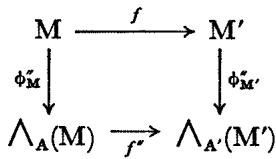
\includegraphics[keepaspectratio]{images/part003_899f4c21.jpg}}

和 \(f''\) 是分次代数同态。立即可以推出，如果 \(\sigma: A' \to A''\) 是另一个环同态， \(M''\) 一个 \(A''\) -模， \(g: M' \to M''\) 一个 \(A'\) -同态（相对于 \(\sigma\) ) 且 \(g'': \bigwedge_{A'}(M') \to \bigwedge_{A''}(M'')\) 相应的 \(A''\) -代数的同态，则复合的代数 A-同态

\[
\bigwedge_ {\mathbf {A}} (\mathbf {M}) \xrightarrow {f ^ {\prime \prime}} \bigwedge_ {\mathbf {A} ^ {\prime}} (\mathbf {M} ^ {\prime}) \xrightarrow {g ^ {\prime \prime}} \bigwedge_ {\mathbf {A} ^ {\prime \prime}} (\mathbf {M} ^ {\prime \prime})\tag{13}
\]

对应于复合 A-同态 \(g \circ f: \mathbf{M} \to \mathbf{M}''\) （相对于 \(\sigma \circ \rho\) ）。

命题 8. 设 A、B 为两个交换环， \(\rho: A \to B\) 一个环同态，且 M 是一个 A-模。典范扩张

\[
\psi : \bigwedge_ {\mathbf {B}} (\mathbf {B} \otimes_ {\mathbf {A}} \mathbf {M}) \rightarrow \mathbf {B} \otimes_ {\mathbf {A}} \bigwedge_ {\mathbf {A}} (\mathbf {M})
\]

的典范扩张是一个分次 B-代数同构，这里所指的 B-线性映射是 \(l_{B} \otimes \phi_{M}^{\prime\prime}: B \otimes_{A} M \to B \otimes_{A} \bigwedge_{A}(M)\) 。

证明源自 §5 第 4 号命题 5 的证明，只需将 T 换为 \(\bigwedge\) ，并将 \(\phi_{\mathbf{M}}\) 换为 \(\phi_{\mathbf{M}}^{\prime \prime}\) 。

\subsection{外代数的正向极限}

设 \((\mathbf{A}_{\alpha},\phi_{\beta \alpha})\) 为交换环的一个有向正向系统， \((\mathbf{M}_{\alpha},f_{\beta \alpha})\) 为 \(\mathbf{A}_{\alpha}\) -模的一个正向系统， \(\mathbf{A} = \varinjlim \mathbf{A}_{\alpha}\) 与 \(\mathbf{M} = \varinjlim \mathbf{M}_{\alpha}\) 。对于 \(\alpha \leqslant \beta\) ，我们由 \(\mathbf{A}_{\alpha}\) -同态 \(f_{\beta \alpha}: \overrightarrow{\mathbf{M}_{\alpha}} \to \mathbf{M}_{\beta}\) 典范地导出一个 \(\mathbf{A}_{\alpha}\) -代数同态（第 5 号，公式 (12)） \(f_{\beta \alpha}^{\prime \prime}: \bigwedge_{\mathbf{A}_{\alpha}} (\mathbf{M}_{\alpha}) \to \bigwedge_{\mathbf{A}_{\beta}} (\mathbf{M}_{\beta})\) ，并且由 (13) 可知 \((\bigwedge_{\mathbf{A}_{\alpha}} (\mathbf{M}_{\alpha}), f_{\beta \alpha}^{\prime \prime})\) 是分次 \(\mathbf{A}_{\alpha}\) -模的一个正向系统。另一方面，设 \(f_{\alpha}: \mathbf{M}_{\alpha} \to \mathbf{M}\) 为典范 \(\mathbf{A}_{\alpha}\) -同态；我们（由第 5 号，公式 (12)）导出一个分次 \(\mathbf{A}_{\alpha}\) -代数同态 \(f_{\alpha}^{\prime \prime}: \bigwedge_{\mathbf{A}_{\alpha}} (\mathbf{M}_{\alpha}) \to \bigwedge_{\mathbf{A}} (\mathbf{M})\) ，并且由 (13) 同样得出 \(f_{\alpha}^{\prime \prime}\) 构成 \(\mathbf{A}_{\alpha}\) -同态的一个正向系统。

命题9. A-同态 \(f'' = \varinjlim f_{\alpha}' : \varinjlim \bigwedge_{A_{\alpha}}(M_{\alpha}) \to \bigwedge_{A}(M)\) 是一个分次代数同构。

证明与 §5 第 4 号命题 6 的证明相同，只需将其中所有的 T 换为 \(\bigwedge\) ，将 \(\phi\) 换为 \(\phi''\) ，并注意到交错代数的正向极限仍是交错的。

\subsection{直和的外代数。分次模的外代数}

设 A 为一个交换环， \(M = \bigoplus_{\lambda \in L} M_{\lambda}\) 为一族 A-模的直和，以及 \(j_{\lambda}: M_{\lambda} \to M\) 为典范单射；由此导出一个分次代数的 A-同态 \(\bigwedge(j_{\lambda}): \bigwedge(M_{\lambda}) \to \bigwedge(M)\) 。由于 \(\bigwedge(M)\) 是反交换的，§4 第 7 号命题 10（或在必要时推广到 L 为无限的情形，参见 §4 第 8 号注记 1）可应用于同态 \(\bigwedge(j_{\lambda})\) ；则存在唯一的代数同态

\[
g \colon \bigotimes_ {\lambda \in L} ^ {g} \Lambda (M _ {\lambda}) \to \Lambda (M)\tag{14}
\]

（也记作 \(g_{\mathbf{M}}\) ）使得 \(\bigwedge (j_{\lambda}) = g \circ f_{\lambda}\) ，其中

\[
f _ {\lambda}: \bigwedge (\mathrm{M} _ {\lambda}) \rightarrow \bigotimes_ {\lambda \in L} ^ {g} \bigwedge (\mathrm{M} _ {\lambda})
\]

表示典范同态。

命题10. 典范同态 \(g\) （公式（14））是分次代数同构。

为了证明 \(g\) 是双射，我们定义一个分次代数同态

\[
h: \bigwedge (\mathbf {M}) \rightarrow \bigotimes_ {\lambda \in L} ^ {\mathfrak {g}} \bigwedge (\mathbf {M} _ {\lambda})\tag{15}
\]

使得 \(g \circ h\) 与 \(h \circ g\) 分别是 \(\bigwedge(\mathbf{M})\) 与 \(\bigotimes_{\lambda \in L} \bigwedge(\mathbf{M}_{\lambda})\) 上的恒等映射。对于每个 \(\lambda \in L\) ，考虑复合线性映射

\[
u _ {\lambda}: \mathrm{M} _ {\lambda} \xrightarrow {\phi_ {\mathrm{M} _ {\lambda}} ^ {n}} \bigwedge (\mathrm{M} _ {\lambda}) \xrightarrow {f _ {\lambda}} \mathbf {g} _ {\lambda \in L} \bigotimes \bigwedge (\mathrm{M} _ {\lambda}).
\]

存在且仅存在一个 A-线性映射 \(u: \mathbf{M} \to {}^{\mathfrak{g}} \bigotimes_{\lambda \in L} \bigwedge (\mathbf{M}_{\lambda})\) ，使得 \(u \circ j_{\lambda} = u_{\lambda}\) （对所有 \(\lambda \in L\) ）。斜张量积 \({}^{\mathfrak{g}} \bigotimes_{\lambda \in L} \bigwedge (\mathbf{M}_{\lambda})\) 是一个交错代数：当 L 有限时，这由 §4 第 9 号命题 14 得出；当 L 任意时，这由 §4 第 8 号注记 1 中给出的该乘积的定义以及交错分次代数的正向极限是交错的这一事实得出。由于 \(u(\mathbf{M})\) 也包含在分次代数 \(\bigotimes_{\lambda \in L} \bigwedge (\mathbf{M}_{\lambda})\) 中次数为1的元素子模中，由第1号命题1和注记1可知，存在唯一的分次代数同态。

\[
h: \bigwedge (\mathbf {M}) \rightarrow \bigotimes_ {\lambda \in L} ^ {\mathfrak {g}} \bigwedge (\mathbf {M} _ {\lambda})
\]

使得 \(h \circ \phi_{\mathbf{M}}'' = u\) 。 \(g \circ h\) 与 \(h \circ g\) 为恒等映射这一事实的验证，与 §6 第 6 号命题 9 中的做法相同，只需将 \(\mathbf{S}\) 换为 \(\bigwedge\) ，将 \(\phi'\) 换为 \(\phi''\) 。

注记。设 \(N = \bigoplus_{\lambda \in L} N_{\lambda}\) 为以 L 为指标集的另一族 A-模的直和，并且对所有 \(\lambda \in L\) ，设 \(v_{\lambda}: M_{\lambda} \to N_{\lambda}\) 为一个 A-线性映射，于是存在 A-线性映射 \(v = \bigoplus_{\lambda} v_{\lambda}: M \to N\) （II，§1，第 6 号，命题 7）。则图表

\[
\begin{array}{c c c} \mathbf {g} _ {\lambda \in L} ^ {\otimes} \wedge (\mathrm{M} _ {\lambda}) & \xrightarrow {g _ {\mathrm{M}}} & \wedge (\mathrm{M}) \\ \bigotimes_ {\lambda \in L} \wedge (v _ {\lambda}) \Big \downarrow & & \Big \downarrow \wedge (v) \\ \mathbf {g} _ {\lambda \in L} ^ {\otimes} \wedge (\mathrm{N} _ {\lambda}) & \xrightarrow {g _ {\mathrm{N}}} & \wedge (\mathrm{N}) \end{array}
\]

是交换的（参见第4节第5号命题8的推论）。

\(\mathbf{g}_{\lambda \in L}^{\otimes} \bigwedge (\mathbf{M}_{\lambda})\) 的 A-子模（ \(\bigwedge^{n}(\mathbf{M})\) 借助同构 \(g\) 与之等同者）可以得到更精确的描述。对每个有限子集 \(J\) （ \(L\) 的），我们记 \(\mathrm{E}_{J} = \mathbf{g}_{\lambda \in J}^{\otimes} \bigwedge (\mathbf{M}_{\lambda})\) ，从而 \(\mathbf{g}_{\lambda \in L}^{\otimes} \bigwedge (\mathbf{M}_{\lambda}) = \lim_{\lambda \to 0} \mathrm{E}_{J}\) 相对于有向集 \(\mathfrak{F}(L)\) （ \(L\) 的有限子集组成的）成立，这是依据定义（§ 4，第 8 号，注记 1）。对每个族 \(\nu = (n_{\lambda}) \in \mathbf{N}^{(L)}\) （从而具有有限支集），它满足 \(\sum_{\lambda \in L} n_{\lambda} = n\) ；对每个有限子集 \(J\) （ \(L\) 的、包含族 \(\nu\) 的支集者），我们记

\[
\bigwedge^ {J, v} (\mathbf {M}) = \bigotimes_ {\lambda \in J} \bigwedge^ {n _ {\lambda}} (\mathbf {M} _ {\lambda})\tag{16}
\]

使得子模 \(\mathbf{E}_{\mathbf{J},n}\) ——即次数 \(n\) 的元素在 \(\mathbf{E}_{\mathbf{J}}\) 中组成的子模——是诸 \(\bigwedge^{\mathbf{J},\nu}(\mathbf{M})\) 的直和，这里族 \(\nu\) 的支集包含于 \(\mathbf{J}\) 且使得

\[
\sum_ {\lambda \in L} n _ {\lambda} = n
\]

（§ 4，第 7 号，命题 10 及第 8 号）。按约定，我们记 \(\bigwedge^{J,\nu}(\mathbf{M}) = \{0\}\) （对族 \(\nu\) ，其支集不包含于 \(J\) ）；于是

\(E_{J,n}\) 也可称为所有 \(\bigwedge^{J,\nu}(M)\) 的直和，其中 \(\nu\) 遍历集合 \(H_n\) ，即所有族 \(\nu = (n_\lambda)_{\lambda \in L}\) （满足 \(\sum_{\lambda \in L} n_\lambda = n\) 者）组成的集合。由于 \(\bigwedge^0(M_\lambda)\) 与 A 等同，显然对 L 的两个有限子集 \(J \subset J'\) 以及支集包含于 J 的族 \(\nu\) ，典范映射 \(\bigwedge^{J,\nu}(M) \to \bigwedge^{J',\nu}(M)\) （即典范映射 \(E_J \to E_{J'}\) 在 \(\bigwedge^{J,\nu}(M)\) 上的限制）是双射。如果对所有 \(\nu \in H_n\) ，

\[
\bigwedge^ {\nu} (\mathbf {M}) = \varinjlim \bigwedge^ {J, \nu} (\mathbf {M})\tag{17}
\]

于是可见，考虑到 II，§ 6，第 2 号，命题 5，我们有：

推论. A-模 \(\bigwedge^{n}(\mathbf{M})\) 是 \(\bigotimes_{\lambda \in L} \bigwedge (\mathbf{M}_{\lambda})\) 的一个子模在同构 (14) 下的像，该子模是诸子模 \(\bigwedge^{\nu}(\mathbf{M})\) 的直和，其中族 \(\nu = (n_{\lambda}) \in \mathbf{N}^{(L)}\) 满足 \(\sum_{\lambda \in L} n_{\lambda} = n\) ；若 \(J\) 是 \(\nu, \bigwedge^{\nu}(\mathbf{M})\) 的支集，则它典范同构于 \(\bigotimes_{\lambda \in J} \bigwedge^{n_{\lambda}}(\mathbf{M}_{\lambda})\) .

一般将 \(\bigwedge^{\nu}(\mathbf{M}),\bigotimes_{\lambda \in J}\bigwedge^{n_{\lambda}}(\mathbf{M}_{\lambda})\) 与它们在 \(\bigwedge^n (\mathbf{M})\) 中的像等同起来。按此约定：

命题11. 设 \(\Delta\) 为交换幺半群， \(\mathbf{M}\) 为类型 \(\Delta\) 的分次 A-模， \((\mathbf{M}_{\alpha})_{\alpha \in \Delta}\) 为其分次。对于每个有序对 \((\alpha, n) \in \Delta \times \mathbf{N}\) ，设 \(\bigwedge^{\alpha, n}(\mathbf{M})\) 为 \(\bigwedge^n (\mathbf{M})\) 的这样的子模：它是诸子模 \(\bigotimes_{\lambda \in J} \bigwedge^{n_{\lambda}}(\mathbf{M}_{\alpha_{\lambda}})\) 的直和，其中 \((n_{\lambda})_{\lambda \in L}\) 遍历整数 \(\geqslant 0\) 的、满足 \(\sum_{\lambda \in L} n_{\lambda} = n\) 的族所成的集合， \(J\) 为其支集，且对于每个 \((n_{\lambda})\) , \((\alpha_{\lambda})_{\lambda \in J}\) 遍历 \(\Delta^J\) 中满足 \(\sum_{\lambda \in J} \alpha_{\lambda} = \alpha\) 的族所成的集合。则 \((\bigwedge^{\alpha, n}(\mathbf{M}))_{(\alpha, n) \in \Delta \times N}\) 是唯一的类型为 \(\Delta \times N\) 、与 \(\bigwedge(\mathbf{M})\) 上的代数结构相容并且在 \(\mathbf{M} = \bigwedge^1 (\mathbf{M})\) 上诱导出给定分次的分次。

\(\bigwedge (\mathbf{M})\) 是诸 \(\bigwedge^{\alpha ,n}(\mathbf{M})\) 的直和这一事实由命题 10 的推论得出；证明的其余部分与 §5 第 5 号命题 7 的证明结尾完全相同。

\subsection{自由模的外代数}

定理1. 设M是一个具有基的A-模 \((e_{\lambda})_{\lambda \in L}\) 。设 L 被赋予全序集的结构（集合论，III，§2，第 3 号，定理 1），并且对于 L 的每个有限子集 J，我们记

\[
e _ {J} = e _ {\lambda_ {1}} \wedge e _ {\lambda_ {2}} \wedge \dots \wedge e _ {\lambda_ {n}}\tag{18}
\]

（其中 \((\lambda_k)_{1 \leqslant k \leqslant n}\) 是 \(J\) 的元素按递增顺序排列的序列（集合论，III，§5，第 3 号，命题 6）；我们记 \(e_\varphi = 1\) ，即 A 的单位元。则诸 \(e_J\) （其中 \(J\) 遍历有限子集组成的集合 \(\mathfrak{F}(L)\) （ \(L\) 的））构成外代数 \(\bigwedge(M)\) 的一组基。

由于 \(e_{\lambda}\) 生成 A-模 M， \(\bigwedge(\mathbf{M})\) 的每个元素都是有限个 \(e_{\lambda}\) 之乘积的线性组合，从而（考虑到第 3 号命题 5）是有限个元素 \(e_{J}\) （ \(J \in \mathfrak{F}(L)\) ）的线性组合。剩下要证明 \(e_{J}\) 在 A 上线性无关。否则，这些元素之间将存在一个系数不全为零的线性关系；此关系中诸 \(e_{J}\) （其系数 \(\neq 0\) 者）所对应的子集 J 的并是 L 的一个有限子集 K（因为系数 \(\neq 0\) 的只有有限个）。设 N 为 M 的由诸 \(e_{\lambda}\) （满足 \(\lambda \in K\) 者）生成的子模；N 是 M 的一个直因子，因此（第 2 号） \(\bigwedge(\mathbf{N})\) 等同于 \(\bigwedge(\mathbf{M})\) 的一个子代数，并且，如果我们证明诸 \(e_{J}\) （ \(J \subset K\) ）构成 \(\bigwedge(\mathbf{N})\) 的一组基，我们将得到所期望的矛盾。

因此，问题归结为在 M 的基为有限时证明定理 1；于是我们可以假设 \(L = [1, m] \subset N\) 。对于每个 \(i \in L\) ，设 \(M_i\) 为 M 的自由子模 \(Ae_i\) ；M 是诸 \(M_i\) 的直和，而 \(\bigwedge(M_i)\) 是 \(\bigwedge^0(M_i) = A\) 与 \(\bigwedge^1(M_i) = M_i\) （第 3 号，命题 6）的直和。令 \(\bigwedge(M)\) 与诸 \(\bigwedge(M_i)\) 的张量积这一 A-模（第 7 号，命题 10）典范地等同；后者以诸基 \((1, e_i)\) （诸 \(\bigwedge(M_i)\) 的基）的张量积为基（II，§ 3，第 7 号，命题 7 的推论 2）；因此我们得到所有元素

\[
u _ {1} \otimes u _ {2} \otimes \dots \otimes u _ {m}
\]

其中 \(u_{i}=1\) 或 \(u_{i}=e_{i}\) ；若 J 是使得 \(u_{i}=e_{i}\) 的指标 i 组成的集合，则 \(u_{1}\otimes u_{2}\otimes\cdots\otimes u_{m}\) 与 \(e_{J}\) 等同，这就完成了证明。

推论 1. 假设 \(\mathbf{L} = [1, m]\) ；则基 \((e_{\mathrm{J}})_{\mathrm{J} \in \mathfrak{P}(\mathrm{L})}\) （ \(\bigwedge (\mathbf{M})\) 的）有 \(2^{m}\) 个元素。对于 \(p > m\) , \(\bigwedge^{p}(\mathbf{M}) = \{0\}\) ； \(\bigwedge^{m}(\mathbf{M})\) 有由单个元素 \(e_{\mathrm{L}}\) 组成的基；对于 \(0 \leqslant p \leqslant m\) ，基 \((e_{\mathrm{J}})\) （ \(\bigwedge^{p}(\mathbf{M})\) 的、由诸 \(e_{\mathrm{J}}\) （满足 \(\operatorname{Card}(\mathbf{J}) = p\) 者）组成的）的元素个数是

\[
\binom {m} {p} = \frac {m !}{p ! (m - p) !}.
\]

这可由《集合论》III，§3，第5号，命题12以及《集合论》III，§5，第8号，命题11的推论1得出。

我们回到定理 1 中集合 L 为任意的情形，并明确给出基 \((e_{J})\) 的乘法表（§1，第 7 号）。给定两个有限子集 \(J\) , \(K\) （全序集 \(L\) 的），我们记

\[
\left\{ \begin{array}{l l} \rho_ {J, K} = 0 & \text { if } J \cap K \neq \varnothing \\ \rho_ {J, K} = (- 1) ^ {\nu} & \text { if } J \cap K = \varnothing \end{array} \right.\tag{19}
\]

其中 v 表示有序对 \((\lambda, \mu) \in J \times K\) 中满足 \(\lambda > \mu\) 者的个数。于是，第 2 号命题 4 的推论 1 立即蕴含关系

\[
e _ {J} \wedge e _ {K} = \rho_ {J, K} e _ {J \cup K}.\tag{20}
\]

注意公式

\[
\rho_ {J, K} \rho_ {K, J} = (- 1) ^ {j k}\tag{21}
\]

当 \(\mathbf{J} \cap \mathbf{K} = \varnothing, j = \operatorname{Card}(\mathbf{J}), k = \operatorname{Card}(\mathbf{K})\) (第3号，命题5之推论2。)

推论2. 若M是投射A-模， \(\bigwedge (\mathbf{M})\) 是投射 A-模。

证明与第5节第5号定理1的推论相同，只需将T替换为 \(\Lambda\) .

推论3. 设 M 为投射 A-模，且 \((x_{i})_{1\leqslant i\leqslant n}\) 为 M 的元素组成的有限序列。要在 M 上存在一个交错 \(n\) -线性形式 \(f\) ，使得

\[
f (x _ {1}, x _ {2}, \dots , x _ {n}) \neq 0,
\]

其充要条件是 \(x_{1} \wedge x_{2} \wedge \cdots \wedge x_{n} \neq 0\) .

我们已经知道（在对 M 不作任何假设的情况下）该条件是必要的（第 4 号，命题 7）。现在假设 M 是投射的，并且

\[
x _ {1} \wedge x _ {2} \wedge \dots \wedge x _ {n} \neq 0.
\]

那么 \(\bigwedge^n (\mathbf{M})\) 是投射的（推论 2），因此典范映射

\[
\bigwedge^ {n} (\mathbf {M}) \rightarrow (\bigwedge^ {n} (\mathbf {M})) ^ {* *}
\]

是单射的（II，§2，第7号，命题13的推论4）；我们由此得出结论，存在一个线性形式 \(g: \bigwedge^{n}(\mathbf{M}) \to \mathbf{A}\) ，使得 \(g(x_{1} \wedge x_{2} \wedge \dots \wedge x_{n}) \neq 0\) 。若 \(f\) 是交错 \(n\) -线性形式中与 \(g\) 相对应的那一个（第 4 号，命题 7），则 \(f(x_{1}, \ldots, x_{n}) \neq 0\) .

\subsection{线性无关的判定准则}

命题12. 设M是一个投射A-模。对于M中的元素 \(x_1, x_2, \ldots, x_n\) 线性相关，必要且充分条件是存在 \(\lambda \neq 0\) ，以及

\[
\lambda x _ {1} \wedge x _ {2} \wedge \dots \wedge x _ {n} = 0.\tag{22}
\]

该条件是必要的（对 M 不作任何假设），因为例如若 \(\lambda x_{1}\) （其中 \(\lambda \neq 0\) ）是 \(x_{2}, \ldots, x_{n}\) 的线性组合，则关系式 (22) 成立（第 3 号，命题 5）。我们通过对 n 作归纳来证明该条件是充分的；对于 n = 1，它是定义的一个平凡推论。因此假设 n \textgreater{} 1 且条件 (22) 对某个 \(\lambda \neq 0\) 成立。若

\[
\lambda x _ {2} \wedge x _ {3} \wedge \dots \wedge x _ {n} = 0,
\]

成立，则归纳假设蕴含 \(x_{2},\ldots,x_{n}\) 线性相关，从而当然 \(x_{1},x_{2},\ldots,x_{n}\) 也线性相关。若 \(\lambda x_{2}\wedge x_{3}\wedge\cdots\wedge x_{n}\neq0\) ，则由第 8 号定理 1 的推论 3 可知，存在一个交错的 \((n-1)\) -线性形式 f 使得 \(f(\lambda x_{2}\wedge x_{3}\wedge\cdots\wedge x_{n})=\mu\neq0\) 。由于

\[
x _ {1} \wedge (\lambda x _ {2}) \wedge \dots \wedge x _ {n} = 0,
\]

由第 8 号定理 1 的推论 3 可知， \(\mu x_{1}\) 是 \(\lambda x_{2}, x_{3}, \ldots, x_{n}\) 的线性组合；因此 \(x_{1}, x_{2}, \ldots, x_{n}\) 线性相关。

推论. 设M和N是两个投射A-模，且 \(f:M\to N\) 是一个A-线性映射。若f是单射，则 \(\bigwedge(f):\bigwedge(\mathbf{M})\to\bigwedge(\mathbf{N})\) 是单射。

我们首先在M是自由的假设下证明这一点；设 \((e_{\lambda})_{\lambda \in L}\) 是M的一组基，从而 \((e_{J})_{J \in \mathfrak{F}(L)}\) （公式(18)）是 \(\bigwedge(M)\) 的一组基。假设 \(\bigwedge(f)\) 的核包含一个元素 \(u = \sum_{J} \alpha_{J} e_{J} \neq 0\) 。设K是使得 \(\alpha_{J} \neq 0\) 的有限子集J中极小者，并设H是L的一个与K不相交的有限子集，使得 \(K \cup H\) 包含所有（有限个）使得 \(\alpha_{J} \neq 0\) 的 J ；于是对所有满足 \(J \neq K\) 且 \(\alpha_{J} \neq 0\) 的 J ，按定义我们有 \(J \cap H \neq 0\) ，从而（第 8 号，公式 (20)）

\[
u \wedge e _ {\mathrm{H}} = + \alpha_ {\mathbf {K}} e _ {\mathbf {K} \cup \mathbf {H}}
\]

属于 \(\bigwedge (\mathbf{M})\) 的双边理想，即 \(\bigwedge (f)\) 的核。我们记 \(e_{\mathbf{K} \cup \mathbf{H}} = e_{\lambda_1} \wedge e_{\lambda_2} \wedge \dots \wedge e_{\lambda_n}\) ；于是 \(\alpha_{\mathbf{K}} f(e_{\lambda_1}) \wedge f(e_{\lambda_2}) \wedge \dots \wedge f(e_{\lambda_n}) = 0\) ；根据命题 12，N 中的元素 \(f(e_{\lambda_i})\) ( \(1 \leqslant i \leqslant n\) ) 线性相关。但这与假设 \(f\) 是单射（II，§1，第11号，命题17的推论3）相矛盾。

现在我们考虑一般情形；设 \(\mathbf{M}'\) 是一个A-模，使得 \(\mathbf{M} \oplus \mathbf{M}' = \mathbf{P}\) 是自由的（II，§2，第2号，命题4）。考虑线性映射 \(g: \mathbf{M} \oplus \mathbf{M}' \to \mathbf{N} \oplus \mathbf{M} \oplus \mathbf{M}'\) ，它使得 \(g(x, y) = (f(x), 0, y)\) ，从而有交换图

\pandocbounded{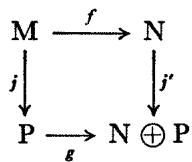
\includegraphics[keepaspectratio]{images/part004_a147f11a.jpg}}

其中竖直箭头是典范单射。由于g是单射且P是自由的， \(\bigwedge(g)\) 如上所见是一个单射同态。现在， \(\bigwedge(j):\bigwedge(\mathbf{M})\to\bigwedge(\mathbf{P})\) 是一个单射同态，因为M是P的一个直因子（第2号）。复合同态

\[
\bigwedge (\mathbf {M}) \xrightarrow {\bigwedge (j)} \bigwedge (\mathbf {P}) \xrightarrow {\bigwedge (g)} \bigwedge (\mathbf {N} \oplus \mathbf {P})
\]

因此是单射的，并且由于它也等于复合同态

\[
\Lambda (\mathbf {M}) \xrightarrow {\Lambda (f)} \Lambda (\mathbf {N}) \xrightarrow {\Lambda (j ^ {\prime})} \Lambda (\mathbf {N} \oplus \mathbf {P})
\]

我们得出结论 \(\bigwedge (f)\) 是单射。

命题13. 设 M 是一个 A-模，N 是 M 的一个直因子子模，它是维数为 p 的自由模，且 \(\{u\}\) 是 \(\bigwedge^{p}(\mathbf{N})\) 的一组基。对于元素 \(x \in M\) 属于 N，必要且充分条件是 \(u \wedge x = 0\) .

设P是M中与N互补的子模，且设 \(y \in N\) , \(z \in P\) 使得 \(x = y + z\) 。则 \(u \wedge x = u \wedge z\) 。由于 \(\bigwedge^{p}(N)\) 是维数为 1 的自由模，映射 \(\phi: P \to P \otimes \bigwedge^{p}(N)\) （它由 \(\phi(p) = p \otimes u\) 给出）是双射（II，§3，第 4 号，命题 4）。另一方面（第7号，命题10），典范同态的复合

\[
\psi : \mathrm{P} \otimes \bigwedge^ {p} (\mathrm{N}) \rightarrow \bigwedge (\mathrm{P}) \otimes \bigwedge (\mathrm{N}) \rightarrow \bigwedge (\mathrm{M})
\]

是单射的。映射 \(\psi \circ \phi\) 因此是单射的，从而命题得证。

定理2. 设 \(\mathbf{M}\) 是一个具有有限基 \((e_i)_{1\leqslant i\leqslant n}\) 的A-模。对于序列 \((x_i)_{1\leqslant i\leqslant n}\) （ \(n\) 个属于 \(\mathbf{M}\) 的元素）构成 \(\mathbf{M}\) 的一个基，必要且充分条件是使得下式成立的元素 \(\lambda \in \mathbf{A}\)

\[
x _ {1} \wedge x _ {2} \wedge \dots \wedge x _ {n} = \lambda . e _ {1} \wedge e _ {2} \wedge \dots \wedge e _ {n}\tag{23}
\]

在 A 中可逆。

请回忆 \(e_{1} \wedge e_{2} \wedge \cdots \wedge e_{n}\) 是 \(\bigwedge^{n}(\mathbf{M})\) 的一个基中的唯一元素（第 8 号，定理 1 的推论 1），因而满足 (23) 的元素 \(\lambda \in A\) 被唯一确定。若 \((x_{i})_{1 \leqslant i \leqslant n}\) 是 M 的一组基，则 \(x_{1} \wedge x_{2} \wedge \cdots \wedge x_{n}\) 是 \(\bigwedge^{n}(\mathbf{M})\) 的一个基中的唯一元素（第 8 号），于是 \(\lambda\) 是可逆的。反之，假设 \(\lambda\) 是可逆的；那么对应于线性映射 \(g: \bigwedge^{n}(\mathbf{M}) \to \mathbf{A}\) （它使得

\[
g (e _ {1} \wedge e _ {2} \wedge \dots \wedge e _ {n}) = \lambda^ {- 1}
\]

）的交错 n-线性形式 f 满足 \(f(x_{1}, x_{2}, \ldots, x_{n}) = 1\) 。对于所有 \(x \in \mathbf{M}\) ，显然

\[
x \wedge x _ {1} \wedge \dots \wedge x _ {n} = 0
\]

（第 3 号，命题 6）；将第 8 号，定理 1 的推论 3 应用于此，我们得到

\[
f (x _ {1}, x _ {2}, \dots , x _ {n}). x = \sum_ {i = 1} (- 1) ^ {i - 1} f (x, x _ {1}, \dots , \hat {x} _ {i}, \dots , x _ {n}). x _ {i}.
\]

由于 \(f(x_{1},\ldots ,x_{n}) = 1\) ，这表明每一个 \(x\in \mathbf{M}\) 都是 \(x_{1},x_{2},\ldots ,x_{n}\) 的线性组合，且由于它们线性无关（因为

\[
x _ {1} \wedge x _ {2} \wedge \dots \wedge x _ {n} \neq 0),
\]

它们构成M的一组基。

\section{行列式}

\subsection{自同态的行列式}

设 M 是一个具有 n 个元素的有限基的 A-模，u 是 M 的一个自同态。A-模 \(\bigwedge^{n}(\mathbf{M})\) 是一个单生成自由模，即与A同构（第8号，定理1的推论1）。 \(\bigwedge^{n}(u)\) 是该模的一个自同态，因此是一个位似 \(z \mapsto \lambda z\) ，其位似比 \(\lambda \in A\) 被唯一确定（II，§2，第 3 号，命题 5）。

定义 1. 一个自同态 \(u\) （自由 A-模 \(M\) 的、维数 \(n\) 为有限者；II，§7，第 2 号，命题 3 的推论及注记 1）的行列式，记作 \(\det u\) ，是标量 \(\lambda\) （它使得 \(\bigwedge^{n}(u)\) 是比率为 \(\lambda\) 的位似）.

根据 §7 第 2 号的公式 (4)，det u 是使得下式成立的唯一标量：

\[
u \left(x _ {1}\right) \wedge u \left(x _ {2}\right) \wedge \dots \wedge u \left(x _ {n}\right) = (\det u). x _ {1} \wedge x _ {2} \wedge \dots \wedge x _ {n}\tag{1}
\]

对每个序列 \((x_{i})_{1\leqslant i\leqslant n}\) （ \(n\) 个 M 的元素）成立。如果 \(\det (u) = 1\) ，则称 \(u\) 为幺模的。

命题1.（i）若 \(u\) 和 \(v\) 是两个有限维自由A-模M的自同态，则

\[
\det (u \circ v) = (\det u) (\det v).\tag{2}
\]

\begin{enumerate}
\def\labelenumi{(\roman{enumi})}
\setcounter{enumi}{1}
\tightlist
\item
  \(\operatorname{det}(1_{\mathbf{M}}) = 1\) ；对每个自同构 \(u\) （ \(\mathbf{M}\) 的自同构）， \(\operatorname{det} u\) 在 \(\mathbf{A}\) 中可逆，且
\end{enumerate}

\[
\det (u ^ {- 1}) = (\det u) ^ {- 1}.\tag{3}
\]

若 \(n\) 是 \(\mathbf{M}\) 的维数，则这由关系式 \(\bigwedge^{n}(u \circ v) = (\bigwedge^{n}(u)) \circ (\bigwedge^{n}(v))\) （§ 7，第 2 号，公式 (3)）直接得出。

设 M 为具有有限基 \((e_{i})_{1\leqslant i\leqslant n}\) 的自由 A-模；给定 M 的 n 个元素组成的一个序列 \((x_{i})_{1\leqslant i\leqslant n}\) ，此序列关于给定基 \((e_i)\) 的行列式（当基不致引起混淆时记作 \(\det(x_1, x_2, \ldots, x_n)\) ）是 M 的自同态 \(u\) （它满足 \(u(e_i) = x_i\) ， \(1 \leqslant i \leqslant n\) ）的行列式。于是由公式 (1)

\[
x _ {1} \wedge x _ {2} \wedge \dots \wedge x _ {n} = \det (x _ {1}, x _ {2}, \dots , x _ {n}) e _ {1} \wedge e _ {2} \wedge \dots \wedge e _ {n}\tag{4}
\]

且此关系刻画了映射 \((x_{i})\mapsto\det(x_{1},x_{2},\ldots,x_{n})\) （从 \(\mathbf{M}^{n}\) 到 A）。它表明该映射是一个交错 \(n\) -线性形式。由于根据 §7 第 4 号命题 7，交错 \(n\) -线性形式组成的 A-模典范同构于 \(\bigwedge^{n}(\mathbf{M})\) 的对偶，且 \(\bigwedge^{n}(\mathbf{M})\) 同构于 A，由此可见每个交错 \(n\) -线性形式在 \(\mathbf{M}^{n}\) 上都可以写成

\[
(x _ {1}, \dots , x _ {n}) \mapsto \alpha \det (x _ {1}, x _ {2}, \dots , x _ {n})
\]

对于某个 \(\alpha \in \mathbf{A}\) .

命题2. 设 M 是一个具有有限基 \((e_i)_{1 \leqslant i \leqslant n}\) 的自由 A-模， \(v\) 是 M 的一个自同态。对每个序列 \((x_i)_{1 \leqslant i \leqslant n}\) （由 \(n\) 个 M 的元素组成），

\[
\det (v (x _ {1}), \dots , v (x _ {n})) = (\det v) \det (x _ {1}, \dots , x _ {n}).\tag{5}
\]

若 \(u\) 是 \(M\) 的、使得 \(u(e_i) = x_i\) 对每个 \(i\) 成立的自同态，则

\[
v (x _ {i}) = (v \circ u) (e _ {i})
\]

因此，(5) 由 (2) 得出。

\subsection{有限维自由模自同构的刻画}

定理1. 设M是有限维自由A-模，u是M的一个自同态。以下条件等价：

\begin{enumerate}
\def\labelenumi{(\alph{enumi})}
\item
  u 是双射；
\item
  \(u\) 是右可逆的（II，§1，第 9 号，命题15的推论1）；
\item
  u是左可逆的（II，§1，第9号，命题15的推论2）；
\item
  u 是满射；
\item
  det u 在 A 中可逆。
\end{enumerate}

设 \((e_i)_{1\leqslant i\leqslant n}\) 是 M 的一组基。如果 \(x_{i} = u(e_{i})\) 对于 \(1\leqslant i\leqslant n\) ，则

\[
x _ {1} \wedge x _ {2} \wedge \dots \wedge x _ {n} = (\det u) e _ {1} \wedge e _ {2} \wedge \dots \wedge e _ {n}.
\]

由 §7 第 9 号定理 2 可知， \(x_{i}\) 构成 M 的一组基的必要且充分条件是 \(\det u\) 为 A 的可逆元；这就证明了 (a) 与 (e) 的等价性。注意 (a) 显然蕴含条件 (b)、(c)、(d) 中的每一个；剩下要证的是 (b)、(c)、(d) 中的每一个都蕴含 (e)。现在，若存在 M 的自同态 \(v\) 使得 \(v \circ u = 1_{\mathbf{M}}\) 或 \(u \circ v = 1_{\mathbf{M}}\) ，则 \((\det v)(\det u) = 1\) ，因此 \(\det u\) 在 A 中可逆。若 \(u\) 是满射，则 \(\bigwedge^{n}(u)\) 也是满射（ \(\S 7\) ，第 2 号，命题 3），换言之，A 中比率为 det \(u\) 的位似是满射，这立即蕴含 det \(u\) 可逆。

命题3. 设M是有限维自由A-模。对于M的每个自同态u，下列条件是等价的：

\begin{enumerate}
\def\labelenumi{(\alph{enumi})}
\setcounter{enumi}{5}
\item
  u是单射；
\item
  det u在A中不是零因子。
\end{enumerate}

沿用定理 1 证明中的记号，u 是单射当且仅当 \(x_{i}\) 线性无关。根据 §7 第 9 号命题 12，其必要且充分条件是关系 \(\lambda x_{1} \wedge x_{2} \wedge \cdots \wedge x_{n} = 0\) （其中 \(\lambda \in A\) ）蕴含 \(\lambda = 0\) 。但这等价于 \(\lambda(\det u) = 0\) ，因为 \(e_{1} \wedge \cdots \wedge e_{n}\) 是 \(\bigwedge^{n}(M)\) 的一个基；由此得出命题。

注记. 当A是域时，定理2的条件(e)等价于命题3的条件(g)，因为它们都表示det \(u \neq 0\) 。因此在这种情况下，定理1和命题3的所有条件都是等价的（参见II，§7，第4号，命题9的推论）。

\subsection{方阵的行列式}

定义2. 设 I 是有限集，A 是交换环，X 是环 A 上的 (I, I) 型方阵（II，§10，第 7 号）。A-模 A \(^{I}\) 的自同态 u（它关于 A \(^{I}\) 的典范基的矩阵为 X）的行列式称为 X 的行列式，记作 det X。

若 \(X = (\xi_{ij})_{(i,j) \in I \times I}\) 且 \((e_i)_{i \in I}\) 是 \(A^I\) 的典范基，则自同态 \(u\) 由下式给出

\[
u (e _ {i}) = \sum_ {j \in J} \xi_ {j i} e _ {j}.
\]

当 \(\mathbf{I} = [1, n] \subset \mathbf{N}\) 时，若记 \(x_{i} = u(e_{i})\) （对每个 \(i \in \mathbf{I}\) ），则 \(X\) 的行列式由关系式

\[
x _ {1} \wedge x _ {2} \wedge \dots \wedge x _ {n} = (\det X) e _ {1} \wedge e _ {2} \wedge \dots \wedge e _ {n}\tag{6}
\]

换言之，det X 等于行列式 \(\det(x_{1}, x_{2}, \ldots, x_{n})\) （关于 \(A^{n}\) 的典范基者）。因此：

命题 4. 对于 \(n\) 个向量 \(x_1, \ldots, x_n\) （ \(A^n\) 的），设 \(X(x_1, \ldots, x_n)\) 表示 \(n\) 阶方阵，其第 \(i\) 列为 \(x_i\) （ \(1 \leqslant i \leqslant n\) ）。则映射

\[
(x _ {1}, \dots , x _ {n}) \mapsto \det (X (x _ {1}, \dots , x _ {n}))
\]

（从 \((\mathbf{A}^n)^n\) 到 \(\mathbf{A}\) ）是交错的且 \(n\) -线性的。

特别地，若矩阵有两列相等，则其行列式为零。若对矩阵的列进行置换，则新矩阵的行列式等于原矩阵的行列式乘以 \(\varepsilon_{\sigma}\) 。若将矩阵的某一列加上另一个不同指标的列的标量倍数，则新矩阵的行列式等于原矩阵的行列式。

更一般地，设 M 是有限维数为 n 的自由 A-模，并设 \((e_{i})_{i\in I}\) 是 M 的一组基；对于 M 的每个自同构 u，若 X 是 u 关于基 \((e_{i})\) 的矩阵，则

\[
\det (u) = \det (X)\tag{7}
\]

这由定义直接推出。

当 \(\mathbf{I} = [1, n]\) 时， \(X\) 的行列式也记作

\[
\det (\xi_ {i j}) _ {1 \leqslant i \leqslant n, 1 \leqslant j \leqslant n}
\]

或在不致引起混淆时简记为 \(\operatorname{det}(\xi_{ij})\) ，也可记作

\[
\left| \begin{array}{c c c c c} \xi_ {1 1} & \xi_ {1 2} & \ldots & \xi_ {1 n} \\ \xi_ {2 1} & \xi_ {2 2} & \ldots & \xi_ {2 n} \\ \cdot & \cdot & \cdot & \cdot & \cdot \\ \xi_ {n 1} & \xi_ {n 2} & \ldots & \xi_ {n n} \end{array} \right|
\]

当 \(X = 1\) 时，矩阵 \(X\) 称为幺模的。

例。(1) 空矩阵的行列式等于 1；一阶方阵的行列式等于该矩阵的唯一元素。对于二阶矩阵

\[
\left( \begin{array}{c c} \xi_ {1 1} & \xi_ {1 2} \\ \xi_ {2 1} & \xi_ {2 2} \end{array} \right)
\]

则，在上述记号下，

\[
x _ {1} \wedge x _ {2} = (\xi_ {1 1} e _ {1} + \xi_ {2 1} e _ {2}) \wedge (\xi_ {1 2} e _ {1} + \xi_ {2 2} e _ {2}) = \xi_ {1 1} \xi_ {2 2} e _ {1} ^ {\prime} \wedge e _ {2} + \xi_ {2 1} \xi_ {1 2} e _ {2} \wedge e _ {1}
\]

，因此

\[
\left| \begin{array}{c c} \xi_ {1 1} & \xi_ {1 2} \\ \xi_ {2 1} & \xi_ {2 2} \end{array} \right| = \xi_ {1 1} \xi_ {2 2} - \xi_ {1 2} \xi_ {2 1}.
\]

我们将第 1 号和第 2 号中的一些结果翻译成矩阵的语言：

命题 5. 若 X 和 Y 是交换环 A 上具有相同有限指标集的两个方阵，则

\[
\det (X Y) = (\det X) (\det Y).\tag{8}
\]

\(X\) 可逆的必要且充分条件是 \(\det X\) 为 \(\mathbf{A}\) 的可逆元，且此时

\[
\det (X ^ {- 1}) = (\det X) ^ {- 1}.\tag{9}
\]

这直接由第 1 号命题 1 和第 2 号定理 1 得出。

推论。两个相似的方阵具有相等的行列式。

若 \(P\) 为可逆方阵，则由 (8) 和 (9) 可得 \(\det(PXP^{-1}) = \det X\) 。

命题6. 对于有限阶方阵X的列向量线性无关，其充分必要条件为det X在A中不是零因子。

这由第 2 号命题 3 得出。

\subsection{行列式的计算}

引理1. 设 A 是一个交换环，M 是一个以 \((e_j)_{j \in J}\) 为基的自由 A-模，其中指标集 \(J\) 是全序的。对于每个整数 \(p \leqslant \operatorname{Card}(J)\) 、每个交错 \(p\) -线性函数 \(f: \mathbf{M}^p \to \mathbf{N}\) （其中 \(N\) 是一个 A-模）以及每一族 \(p\) 个元素 \(x_i = \sum_{j \in J} \xi_{ji} e_j\) （属于 \(M\) ； \(1 \leqslant i \leqslant p\) ），

\[
\begin{array}{r l} f (x _ {1}, x _ {2}, \dots , x _ {p}) & = \sum_ {j _ {1} <   j _ {2} <   \dots <   j _ {p}} \left(\sum_ {\sigma \in \mathfrak {S} _ {p}} \varepsilon_ {\sigma}. \xi_ {j _ {\sigma (1)}, 1} \xi_ {j _ {\sigma (2)}, 2} \dots \xi_ {j _ {\sigma (p)}, p}\right) f (e _ {j _ {1}}, \dots , e _ {j _ {p}}) \end{array}\tag{10}
\]

其中 \((j_k)_{1\leqslant k\leqslant p}\) 遍历由 J 的元素组成的 \(p\) 项严格递增序列的集合。

现在

\[
f (x _ {1}, \dots , x _ {p}) = \sum_ {(j _ {k})} \xi_ {j _ {1}, 1} \xi_ {j _ {2}, 2} \dots \xi_ {j _ {p}, p} f (e _ {j _ {1}}, e _ {j _ {2}}, \dots , e _ {j _ {p}})
\]

其中 \((j_k)_{1 \leqslant k \leqslant p}\) 遍历所有 \(p\) 项序列（ \(J\) 的元素组成的）；然后只需将 §7 第 4 号命题 7 的推论 1 应用于 \(f\) 。

特别地，若J是有限的且含有n个元素，且 \(x_{i} = \sum_{j \in J} \xi_{ji} e_{j} (1 \leqslant i \leqslant n)\) 是 M 的 n 个元素，则

\[
\begin{array}{l} \text {(11)} \quad x _ {1} \wedge x _ {2} \wedge \dots \wedge x _ {n} \\ = \left(\sum_ {\sigma \in \mathfrak {S} _ {n}} \varepsilon_ {\sigma} \xi_ {j _ {\sigma (1)}, 1} \xi_ {j _ {\sigma (2)}, 2} \dots \xi_ {j _ {\sigma (n)}, n}\right) e _ {j _ {1}} \wedge e _ {j _ {2}} \wedge \dots \wedge e _ {j _ {n}} \end{array}
\]

其中 \((j_k)_{1\leqslant k\leqslant n}\) 是 J 的 \(n\) 个元素按递增顺序排列成的唯一序列，从而

\[
\det (x _ {1}, x _ {2}, \dots , x _ {n}) = \sum_ {\sigma \in \mathfrak {S} _ {n}} \varepsilon_ {\sigma}. \xi_ {j _ {\sigma (1)}, 1} \xi_ {j _ {\sigma (2)}, 2} \dots \xi_ {j _ {\sigma (n)}, n}.\tag{12}
\]

采用引理1的记号，比较公式(10)和(12)可得

\[
x _ {1} \wedge x _ {2} \wedge \dots \wedge x _ {p} = \sum_ {\mathrm{H} \in \mathfrak {F} _ {p} (J)} \det (x _ {\mathrm{H}, 1}, x _ {\mathrm{H}, 2}, \dots , x _ {\mathrm{H}, p}) e _ {\mathrm{H}}\tag{13}
\]

其中 \(\mathfrak{F}_{p}(\mathrm{J})\) 是 J 的具有 p 个元素的子集组成的集合，并且对每个子集 \(\mathrm{H}\in\mathfrak{F}_{p}(\mathrm{J})\) ，我们记 \(x_{H,i}=\sum_{j\in H}\xi_{ji}e_{j}\) 和 \(e_{H}=e_{j_{1}}\wedge e_{j_{2}}\wedge\cdots\wedge e_{j_{p}},(j_{k})_{1\leqslant k\leqslant p}\) 是 H 的元素按递增顺序排列成的序列；这里约定 \(\det(x_{\mathrm{H},1},\ldots,x_{\mathrm{H},p})\) 是相对于基 \((e_{jk})_{1\leqslant k\leqslant p}\) 取的。

命题7. 设I为有限集，且 \(X = (\xi_{ji})_{(j, i) \in I \times I}\) 为交换环A上的(I, I)型方阵。则

\[
\det X = \sum_ {\sigma \in \mathfrak {S} _ {I}} \varepsilon_ {\sigma} \left(\prod_ {i \in I} \xi_ {\sigma (i), i}\right)\tag{14}
\]

其中 \(\sigma\) 遍历群 \(\mathfrak{S}_{\mathbf{I}}\) （ \(\mathbf{I}\) 的置换组成的群），而 \(\varepsilon_{\sigma}\) 是 \(\sigma\) 的符号（I，§5，第 7 号）。

只需考虑 \(I = [1, n] \subset N\) 的情形，然后只需应用公式 (12)，其中 \((e_{i})_{1 \leqslant i \leqslant n}\) 是 \(A^{n}\) 的典范基，诸 \(x_{i}\) 是 X 的列（参见第 3 号，公式 (6)）。

特别地，对于三阶矩阵的行列式

\[
X = \left( \begin{array}{c c c} \xi_ {1 1} & \xi_ {1 2} & \xi_ {1 3} \\ \xi_ {2 1} & \xi_ {2 2} & \xi_ {2 3} \\ \xi_ {3 1} & \xi_ {3 2} & \xi_ {3 3} \end{array} \right)
\]

我们有

\[
\begin{array}{r l} \det (X) = & \xi_ {1 1} \xi_ {2 2} \xi_ {3 3} + \xi_ {1 2} \xi_ {2 3} \xi_ {3 1} + \xi_ {2 1} \xi_ {3 2} \xi_ {1 3} \\ & - \xi_ {1 3} \xi_ {2 2} \xi_ {3 1} - \xi_ {1 2} \xi_ {2 1} \xi_ {3 3} - \xi_ {1 1} \xi_ {2 3} \xi_ {3 2}. \end{array}
\]

命题 8. 对于交换环上的每个方阵 X，转置矩阵 \(^{t}X\) 的行列式等于 X 的行列式。

假设 X 是 (I, I) 型的。对于每一对有序的置换 \(\sigma\) , \(\tau\) （ \(S_{I}\) 中的；因为乘法是可交换的），

\[
\prod_ {i \in I} \xi_ {\sigma (i), i} = \prod_ {j \in I} \xi_ {\sigma (\tau (j)), \tau (j)}.
\]

特别地取 \(\tau = \sigma^{-1}\) ；利用 \(\varepsilon_{\sigma^{-1}} = \varepsilon_{\sigma}\) 这一事实，可以看出

\[
\det X = \sum_ {\sigma \in \mathfrak {S} _ {I}} \varepsilon_ {\sigma}. \left(\prod_ {i \in I} \xi_ {i, \sigma (i)}\right),\tag{15}
\]

这证明了该命题。

推论 1. 对于 \(n\) 个向量 \(x_1, \ldots, x_n\) （ \(A^n\) 的），设 \(Y(x_1, \ldots, x_n)\) 表示 \(n\) 阶方阵，其第 \(i\) 行为 \(x_i\) （ \(1 \leqslant i \leqslant n\) ）。则映射

\[
(x _ {1}, \dots , x _ {n}) \mapsto \det (Y (x _ {1}, \dots , x _ {n}))
\]

从 \((\mathbf{A}^n)^n\) 到 \(\mathbf{A}\) 是交错的且 \(n\) -线性的。

推论 2. 对于方阵 \(X\) （交换环 \(A\) 上的、阶为有限的），下列条件等价：

\begin{enumerate}
\def\labelenumi{(\roman{enumi})}
\item
  \(X\) 的行是线性无关的；
\item
  \(X\) 的列是线性无关的；
\item
  det X 在 A 中不是零因子。
\end{enumerate}

这直接由第 3 号命题 6 和上述命题 8 得出。

推论3. 设 \(u\) 是有限维自由 A-模 \(M\) 的一个自同态， \({}^t u\) 是对偶模 \(M^*\) 的转置自同态（II，§2，第 5 号，定义 5）；则

\[
\det (t u) = \det (u).\tag{16}
\]

若 X 是 u 关于 M 的一组基的矩阵，则 \({}^{t}X\) 是 \({}^{t}u\) 关于对偶基的矩阵（II，§10，第 4 号，命题 3）；由于 \(\det(u) = \det(X)\) 且 \(\det(^{t}u) = \det(^{t}X)\) ，结论由命题 8 得出。

\subsection{矩阵的子式}

设 \(X\) 是 \((\xi_{ij})_{(i,j)\in I\times J}\) 型为 \((I,J)\) 的长方矩阵，其指标集 \(I\) 和 \(J\) 是全序的。若 \(H\subset I\) 与 \(K\subset J\) 是具有相同个数 \(p\) 个元素的有限子集，则存在唯一的递增双射 \(\phi :H\to K\) （集合论，III，§5，第 3 号，命题 6）；我们用 \(X_{H,K}\) 表示型为 \((H,H)\) 、等于 \((\xi_{i,\phi (j)})_{(i,j)\in H\times H}\) 的方阵。若 \(X\) 的元素属于交换环 \(A\) ，则行列式 \(\det (X_{H,K})\) 称为矩阵 \(X\) 的指标为 \(H,K\) 的子式；这些行列式（对所有有序对 \((H,K)\) 而言，其中 H 和 K 分别是 \(I\) 和 \(J\) 的含 \(p\) 个元素的子集）也称为 \(X\) 的 \(p\) 阶子式。利用这一记号：

命题9. 设 M 是一个具有基 \((e_i)_{i \in J}\) 的 A-模（有限或非有限），其指标集 J 是全序的。对每个整数 \(p > 0\) ，设 \((e_H)_{H \in \mathfrak{F}_p(J)}\) 为 \(\bigwedge^p(M)\) 的相应基（§7，第 8 号）。设 \((x_i)_{1 \leqslant i \leqslant p}\) 是 M 的 \(p\) 个元素组成的一个序列；设

\[
x _ {i} = \sum_ {j \in J} \xi_ {j i} e _ {j} \quad for i \in I = [1, p]
\]

并设 \(X\) 表示 \((\xi_{ji})\) 型为 (J, I) 的矩阵。则

\[
x _ {1} \wedge x _ {2} \wedge \dots \wedge x _ {p} = \sum_ {\mathrm{H} \in \mathfrak {F} _ {p} (J)} (\det X _ {\mathrm{H,I}}) e _ {\mathrm{H}}.\tag{17}
\]

其中 H 遍历集合 \(\mathfrak{F}_{p}(\mathrm{J})\) ，即 J 的具有 p 个元素的子集组成的集合。

这直接由第 4 号的公式 (12) 和第 3 号的公式 (6) 得出。

命题10. 设 M 和 N 是维数分别为 m 和 n 的两个自由 A-模， \(u: \mathbf{M} \to \mathbf{N}\) 是一个线性映射， \(X\) 是 \(u\) 关于 M 的基 \((e_i)_{1 \leqslant i \leqslant m}\) 与 N 的基 \((f_j)_{1 \leqslant j \leqslant n}\) 的矩阵。那么，对每个整数 \(p \leqslant \inf(m, n)\) ， \(\bigwedge^p(u)\) 关于基 \((e_{\mathbf{K}})_{\mathbf{K} \in \mathfrak{F}_p(\mathbf{I})}\) （ \(\bigwedge^p(\mathbf{M})\) 的基）与基 \((f_{\mathrm{H}})_{\mathrm{H} \in \mathfrak{F}_p(\mathrm{J})}\) （ \(\bigwedge^p(\mathbf{N})\) 的基）（其中我们记 \(\mathbf{I} = [1, m]\) 和 \(\mathbf{J} = [1, n]\)）的矩阵是矩阵 \((\det(X_{\mathrm{H},\mathbf{K}}))\) ，其型为 \((\mathfrak{F}_p(\mathbf{J}), \mathfrak{F}_p(\mathbf{I}))\) （因而有 \(\binom{n}{p}\) 行和 \(\binom{m}{p}\) 列）。

对 \(\mathbf{K} \subset \mathbf{J}\) 的含 \(p\) 个元素的子集，令 \((j_k)_{1 \leqslant k \leqslant p}\) 为 \(\mathbf{K}\) 的元素按递增顺序排列成的序列；根据 \(\bigwedge^p(u)\) 的定义及 §7 第 2 号公式 (4)

\[
\bigwedge^ {p} (u) \left(e _ {\mathbf {K}}\right) = u \left(e _ {j _ {1}}\right) \wedge u \left(e _ {j _ {2}}\right) \wedge \dots \wedge u \left(e _ {j _ {p}}\right).
\]

因此， \(\bigwedge^{p}(u)\) 的矩阵中位于指标H所在行与指标K所在列的元素，是元素 \(u(e_{j_1}) \wedge \cdots \wedge u(e_{j_p})\) 的指标H分量；因此由命题9，它等于 \(\det(X_{\mathrm{H},\mathbf{K}})\) 。

矩阵 \((\det(X_{\mathrm{H},\mathbf{K}}))\) 称为矩阵 X 的 p 次外幂，记作 \(\bigwedge^{p}(X)\) 。当 p = m = n 时， \(\bigwedge^{n}(X)\) 是仅含单个元素 \(\det(X)\) 的矩阵。

命题11. 设 M 是维数 n 为有限的自由 A-模；对 M 的每个自同态 u 以及 A 的每一对有序元素 \(\xi\) , \(\eta\) ，

\[
\det (\xi 1 _ {\mathrm{M}} + \eta u) = \sum_ {k \geqslant 0} \operatorname{Tr} \left(\bigwedge^ {k} (u)\right) \xi^ {n - k} \eta^ {k}.\tag{18}
\]

设 \((e_i)_{1\leqslant i\leqslant n}\) 是 M 的一组基，并令 \(\mathbf{I} = [1,n]\) ；为计算 (18) 的左边，我们必须构成乘积

\[
\left(\xi e _ {1} + \eta u (e _ {1})\right) \wedge \left(\xi e _ {2} + \eta u (e _ {2})\right) \wedge \dots \wedge \left(\xi e _ {n} + \eta u (e _ {n})\right)
\]

它等于诸项 \(\xi^{n - p}\eta^{p}z_{\mathbf{K}}\) 之和，其中

\[
z _ {K} = x _ {1} \wedge x _ {2} \wedge \dots \wedge x _ {n}
\]

其中 \(x_{i} = u(e_{i})\) （对 \(i \in \mathbf{K}\) ）， \(x_{i} = e_{i}\) （对 \(i \in \mathbf{H} = \mathbf{I} - \mathbf{K}\) ），这里整数 \(p\) 遍历区间 \([0, n]\) ，而对每个 \(p, \mathbf{K}\) 遍历 I 的具有 p 个元素的子集组成的集合。若 \(i_{1} < i_{2} < \cdots < i_{n-p}\) （相应地， \(j_{1} < j_{2} < \cdots < j_{p}\) ）是 H（相应地，K）的元素按递增顺序排列的结果，则我们可以写出（§7，第 8 号，定理 1 的推论 1 及公式 (19)）

\[
z _ {\mathbf {K}} = \rho_ {\mathrm{H}, \mathbf {K}} e _ {i _ {1}} \wedge e _ {i _ {2}} \wedge \dots \wedge e _ {i _ {n - p}} \wedge u (e _ {j _ {1}}) \wedge \dots \wedge u (e _ {j _ {p}}).
\]

但若 \(X\) 是 \(u\) 关于基 \((e_i)\) 的矩阵，则由命题 10

\[
u (e _ {j _ {1}}) \wedge \dots \wedge u (e _ {j _ {p}}) = \sum_ {\mathrm{L} \in \mathfrak {F} _ {p} (\mathrm{I})} (\det X _ {\mathrm{L}, \mathrm{K}}) e _ {\mathrm{L}}
\]

因此

\[
z _ {\mathbf {K}} = \rho_ {\mathrm{H}, \mathbf {K}} \sum_ {\mathbf {L} \in \mathfrak {F} _ {p} (\mathbf {I})} (\det X _ {\mathbf {L}, \mathbf {K}}) e _ {\mathrm{H}} \wedge e _ {\mathrm{L}}.
\]

现在，除 L = K 的情形外均有 \(H \cap L \neq \varnothing\) ；因此由 §7 第 8 号公式 (20) 得 \(z_{K} = (\det X_{K,K})e_{1} \wedge e_{2} \wedge \cdots \wedge e_{n}\) ，而公式 (18) 随后由命题 10 及矩阵的迹的定义（II，§10，第 11 号，公式 (49) 和 (50)）得出。

推论. 在与命题 11 相同的假设下，对自同态 \(\bigwedge(u)\) （A-模 \(\bigwedge(M)\) 的），

\[
\operatorname{Tr} (\bigwedge (u)) = \det (1 _ {\mathbf {M}} + u).\tag{19}
\]

只需在 (18) 中把 \(\xi\) 和 \(\eta\) 都换成 1，并注意到 \(\bigwedge(u)\) 关于由诸 \(e_{\mathbf{H}}\) （ \(\mathbf{H} \in \mathfrak{F}(\mathbf{I})\) ）组成的基的矩阵，是由诸 \(\bigwedge^{k}(u)\) （ \(k \geqslant 0\) ）的矩阵组成的分块对角矩阵（II，§ 10，第 7 号，例 IV）。

\subsection{行列式的展开}

设 I 是一个全序的有限指标集。对 I 的每个子集 H，令 \(H'\) 表示补集 I - H。令 \(X = (\xi_{ji})\) 是一个 (I, I) 型方阵，它可视为 M = A \(^{I}\) 的某个自同态 u 关于 M 的典范基 \((e_{i})_{i \in I}\) 的矩阵。设 n = Card(I)，并设 H 是 I 的含 \(q \leqslant n\) 个元素的子集，K 是 I 的含 n - q 个元素的子集；那么我们可以写出（第 5 号，命题 10）

\[
\begin{array}{r l} (\bigwedge^ {q} (u)) (e _ {\mathrm{H}}) & = \sum_ {\mathbf {R}} \det (X _ {\mathbf {R}, \mathrm{H}}) e _ {\mathbf {R}} \\ (\bigwedge^ {n - q} (u)) (e _ {\mathbf {K}}) & = \sum_ {\mathbf {S}} \det (X _ {\mathbf {S}, \mathbf {K}}) e _ {\mathbf {S}} \end{array}
\]

其中 R（相应地，S）遍历 I 的具有 q（相应地，n - q）个元素的子集组成的集合。由 §7 第 8 号的公式 (19) 和 (20) 可知

\[
e _ {\mathbf {R}} \wedge e _ {\mathbf {S}} = 0
\]

除非 \(\mathbf{S} = \mathbf{R}'\) ，由此得到公式

\[
\left(\bigwedge^ {q} (u) \left(e _ {\mathrm{H}}\right)\right) \wedge \left(\bigwedge^ {n - q} (u) \left(e _ {\mathrm{K}}\right)\right) = \sum_ {\mathbf {R}} \rho_ {\mathbf {R}, \mathbf {R} ^ {\prime}} \det \left(X _ {\mathbf {R}, \mathbf {H}}\right) \det \left(X _ {\mathbf {R} ^ {\prime}, \mathbf {K}}\right) e _ {\mathbf {I}}\tag{20}
\]

其中 R 遍历集合 \(\mathfrak{F}_{q}(\mathbf{I})\) ，即 I 的具有 q 个元素的子集组成的集合。

若取 \(\mathbf{K} = \mathbf{H}'\) ，则由 \(\bigwedge^{n}(u)\) 的定义（ \(\S 7\) ，第 2 号，公式 (4)）以及 \(\S 7\) 第 3 号命题 5 的推论 1 可知，(20) 的右端为 \(\rho_{\mathrm{H},\mathrm{H}'}\bigwedge^{n}(u)(e_{\mathrm{I}})\) 。因此（第 1 号，公式 (1) 以及 \(\S 7\) ，第 2 号，公式 (4)）

\[
\det (X) = \rho_ {\mathrm{H}, \mathrm{H} ^ {\prime}} \sum_ {\mathbf {R} \in \mathfrak {F} _ {q} (\mathbf {I})} \rho_ {\mathrm{R}, \mathrm{R} ^ {\prime}} \det (X _ {\mathbf {R}, \mathrm{H}}) \det (X _ {\mathbf {R} ^ {\prime}, \mathrm{H} ^ {\prime}}).\tag{21}
\]

另一方面，若 \(\mathbf{K} \neq \mathbf{H}'\) ，则 \(\mathbf{H} \cap \mathbf{K} \neq \varnothing\) ；由于 (20) 的左端为 \(\pm \bigwedge^{n}(u)(e_{\mathbf{H}} \wedge e_{\mathbf{K}})\) ，它为零，从而

\[
\sum_ {\mathbf {R}} \rho_ {\mathbf {R}, \mathbf {R} ^ {\prime}} \det (X _ {\mathbf {R}, \mathbf {H}}) \det (X _ {\mathbf {R} ^ {\prime}, \mathbf {K}}) = 0 \quad \text { for } \mathbf {K} \neq \mathbf {H} ^ {\prime}.\tag{22}
\]

(21) 的右端称为矩阵 \(X\) 的行列式按 \(q\) 列（其指标属于 \(\mathbf{H}\) ）与 \(n - q\) 列（其指标属于 \(\mathbf{H}'\) ，即 \(\mathbf{H}\) 的补集）的拉普拉斯展开。子式 \(\det(X_{\mathbf{R},\mathbf{H}})\) 与 \(\det(X_{\mathbf{R}',\mathbf{H}'})\) 有时称为互补的。

拉普拉斯展开的一个重要而简单的情形是 \(\mathbf{I} = [1, n]\) 且 \(q = 1\) ，从而 \(\mathrm{H} = \{i\}\) ；于是对每个仅含一个元素的子集 \(\mathbf{R} = \{j\}\) （ \(\mathbf{I}\) 的），有 \(\det X_{\mathbf{R},\mathbf{H}} = \xi_{ji}\) 。 \(\det X_{\mathbf{R}',\mathbf{H}'}\) 的子式是由 \(X\) 中删去指标为 \(j\) 的行与指标为 \(i\) 的列所得的矩阵典范地（第 5 号）导出的方阵的行列式。我们把这个方阵记作 \(X^{ji}\) 。显然 \(\rho_{\mathrm{H},\mathrm{H}'} = (-1)^{i-1}\) 且 \(\rho_{\mathrm{R},\mathrm{R}'} = (-1)^{j-1}\) ；因此在此情形下 (21) 变为

\[
\det X = \sum_ {j = 1} ^ {n} (- 1) ^ {i + j} \xi_ {j i} \det (X ^ {j i})\tag{23}
\]

并且我们类似地从 (22) 得到

\[
\sum_ {j = 1} ^ {n} (- 1) ^ {j} \xi_ {j i} \det (X ^ {j k}) = 0 \quad \text { for } k \neq i.\tag{24}
\]

公式 (23) 称为 X 的行列式按指标为 i 的列的展开。标量 \((-1)^{i+j}\det(X^{ji})\) 称为 X 中指标为 j 和 i 的代数余子式（或者，滥用术语，称为 \(\xi_{ji}\) 的代数余子式）。

X 的代数余子式矩阵是矩阵

\[
Y = ((- 1) ^ {i + j} \det (X ^ {j i}))\tag{25}
\]

其第 j 行第 i 列的元素是指标为 j 和 i 的代数余子式。公式 (23) 和 (24) 等价于公式

\[
{ } ^ { t } Y . X = ( \operatorname * { d e t } X ) I _ { n } .\tag{26}
\]

因此：

命题 12. 对每个可逆方阵 \(X\) （型为 \((n, n)\) ）， \(X\) 的逆由公式给出

\[
X ^ {- 1} = (\det X) ^ {- 1}. ^ {t} Y\tag{27}
\]

其中 Y 是 X 的代数余子式矩阵。

通过考虑 X 的转置并利用第 5 号的命题 8，可以得到关于两组互补的行集合的拉普拉斯展开，特别是 det X 按某一行展开的展开式，从而有与

\[
X. ^ {t} Y = (\det X) I _ {n},\tag{28}
\]

在上述记号中等价的公式。

容易验证，若 X 是维数为 n 的自由 A-模 M 的自同态 u 关于基 \((e_{i})_{1\leq i\leq n}\) 的矩阵，则 \(^{t}Y\) 是 M 的自同态 \(\tilde{u}\) 的矩阵，后者由下列条件定义：对 M 中每一组 n 个元素 \(x, y_{2}, \ldots, y_{n}\) ，

\[
\tilde {u} (x) \wedge y _ {2} \wedge \dots \wedge y _ {n} = x \wedge u (y _ {2}) \wedge \dots \wedge u (y _ {n}).
\]

\(\tilde{u}\) 称为 u 的余转置（参见 §11，第 11 号，命题 13 的推论）。

例。（1）范德蒙德行列式。给定序列 \((\zeta_{i})_{1\leqslant i\leqslant n}\) （ \(n\) 个 A 的元素），该序列的范德蒙德行列式是行列式

\[
\mathrm{V} (\zeta_ {1}, \zeta_ {2}, \dots , \zeta_ {n}) = \left| \begin{array}{c c c c} 1 & 1 & \dots & 1 \\ \zeta_ {1} & \zeta_ {2} & \dots & \zeta_ {n} \\ \zeta_ {1} ^ {2} & \zeta_ {2} ^ {2} & \dots & \zeta_ {n} ^ {2} \\ \cdot & \cdot & \cdot & \cdot \\ \zeta_ {1} ^ {n - 1} & \zeta_ {2} ^ {n - 1} & \dots & \zeta_ {n} ^ {n - 1} \end{array} \right|
\]

我们将证明

\[
\mathrm{V} \left(\zeta_ {1}, \zeta_ {2}, \dots , \zeta_ {n}\right) = \prod_ {i <   j} \left(\zeta_ {j} - \zeta_ {i}\right).\tag{29}
\]

由于该命题对 \(n = 1\) 是显然的，我们对 \(n\) 作归纳论证。

对于每个指标 \(k \geqslant 2\) ，我们从指标为 k 的行中减去指标为 k - 1 的行乘以 \(\zeta_{1}\) ；行列式的值不变，因此

\[
\mathrm{V} \left(\zeta_ {1}, \zeta_ {2}, \dots , \zeta_ {n}\right) = \left| \begin{array}{c c c c c c c c c} 1 & 1 & & \dots & 1 \\ 0 & \zeta_ {2} - \zeta_ {1} & & \dots & \zeta_ {n} - \zeta_ {1} \\ 0 & \zeta_ {2} \left(\zeta_ {2} - \zeta_ {1}\right) & & \dots & \zeta_ {n} \left(\zeta_ {n} - \zeta_ {1}\right) \\ . & . & . & . & . & . & . & . & . \\ 0 & \zeta_ {2} ^ {n - 2} \left(\zeta_ {2} - \zeta_ {1}\right) & & \dots & \zeta_ {n} ^ {n - 2} \left(\zeta_ {n} - \zeta_ {1}\right) \end{array} \right|
\]

由此，先按第一列展开，再从如此得到的子式的指标为 k-1 的列中取出因子 \(\zeta_{k}-\zeta_{1}\) （ \(2\leqslant k\leqslant n\) ），得到

\[
\mathrm{V} \left(\zeta_ {1}, \dots , \zeta_ {n}\right) = \left(\zeta_ {2} - \zeta_ {1}\right) \left(\zeta_ {3} - \zeta_ {1}\right) \dots \left(\zeta_ {n} - \zeta_ {1}\right) V \left(\zeta_ {2}, \dots , \zeta_ {n}\right)
\]

这通过归纳法确立了 (29)。

\begin{enumerate}
\def\labelenumi{(\arabic{enumi})}
\setcounter{enumi}{1}
\tightlist
\item
  考虑一个 n 阶方阵，它以“矩阵的上三角矩阵”形式呈现（II，§ 10，第 7 号，例 IV）
\end{enumerate}

\[
X = \left( \begin{array}{c c} Y & T \\ 0 & Z \end{array} \right)
\]

我们证明

\begin{enumerate}
\def\labelenumi{(\arabic{enumi})}
\setcounter{enumi}{29}
\tightlist
\item
\end{enumerate}

\[
\det X = (\det Y) (\det Z).
\]

设 \(n\) 是矩阵 \(X, h\) 的阶，即 \(Y, (e_i)_{1 \leqslant i \leqslant n}\) （ \(A^n\) 的典范基）的阶， \(x_i\) （ \(1 \leqslant i \leqslant n\) ）是 \(X\) 的列；假设蕴含列 \(x_1, \ldots, x_h\) 属于 \(A^n\) 的以 \(e_1, \ldots, e_h\) 为基的子模，于是由定义（第 3 号，公式 (6)）

\[
x _ {1} \wedge x _ {2} \wedge \dots \wedge x _ {h} = (\det Y) e _ {1} \wedge e _ {2} \wedge \dots \wedge e _ {h}.
\]

另一方面，对每个指标 i \textgreater{} h，我们可以写出 \(x_{i} = y_{i} + z_{i}\) ，其中 \(y_{i}\) 是 \(e_{1}, e_{2}, \ldots, e_{h}\) 的线性组合， \(z_{i}\) 是 \(e_{h+1}, \ldots, e_{n}\) 的线性组合。由 (30)， \(x_{1} \wedge x_{2} \wedge \cdots \wedge x_{h} \wedge y_{i} = 0\) 对所有 i \textgreater{} h 成立，因此

\[
x _ {1} \wedge x _ {2} \wedge \dots \wedge x _ {n} = (\det Y) e _ {1} \wedge e _ {2} \wedge \dots \wedge e _ {h} \wedge z _ {h + 1} \wedge \dots \wedge z _ {n}.
\]

但根据定义

\[
z _ {h + 1} \wedge z _ {h + 2} \wedge \dots \wedge z _ {n} = (\det Z) e _ {h + 1} \wedge e _ {h + 2} \wedge \dots \wedge e _ {n}
\]

由此得出公式(30)。

通过对 \(p\) 作归纳可知，若 \(X\) 具有矩阵的上三角矩阵的形式：

\[
X = \left( \begin{array}{c c c c c} X _ {1 1} & X _ {1 2} & \ldots & X _ {1 p} \\ 0 & X _ {2 2} & \ldots & X _ {2 p} \\ \cdot & \cdot & \cdot & \cdot & \cdot \\ 0 & 0 & \ldots & X _ {p p} \end{array} \right)\tag{31}
\]

\[
\det X = (\det X _ {1 1}) (\det X _ {2 2}) \dots (\det X _ {p p}).
\]

这尤其可以应用于三角矩阵（其中所有 \(X_{ii}\) 均为 1 阶）以及更特别地对角矩阵：

\[
\det (\operatorname{diag} \left(\alpha_ {1}, \alpha_ {2}, \dots , \alpha_ {n}\right)) = \alpha_ {1} \alpha_ {2} \dots \alpha_ {n}.\tag{32}
\]

\begin{enumerate}
\def\labelenumi{(\arabic{enumi})}
\setcounter{enumi}{2}
\tightlist
\item
  设M、M'为两个自由A-模，维数分别为n、 \(n'\) ，u为M的一个自同态， \(u'\) 为M'的一个自同态。则
\end{enumerate}

\[
\det (u \otimes u ^ {\prime}) = (\det u) ^ {n ^ {\prime}} (\det u ^ {\prime}) ^ {n}.\tag{33}
\]

因为我们可以写出 \(u \otimes u' = (u \otimes 1_{\mathbf{M}'}) \circ (1_{\mathbf{M}} \otimes u')\) ，然后就归结到两个自同态 \(u, u'\) 之一为恒等映射的情形。例如，若 \(u' = 1_{\mathbf{M}'}\) 且 \(X\) 是 \(u\) 关于一个基 \((e_i)\) （ \(\mathbf{M}\) 的）的矩阵，则 \(u \otimes 1_{\mathbf{M}'}\) 关于 \((e_i)\) 与 \(\mathbf{M}'\) 的一组基的张量积的矩阵，可以写成一个矩阵（具有 \(n'\) 行和 \(n'\) 列），其元素是具有 \(n\) 行和 \(n\) 列的矩阵

\[
\left( \begin{array}{c c c c} X & 0 & \ldots & 0 \\ 0 & X & \ldots & 0 \\ \cdot & \cdot & \cdot & \cdot \\ 0 & 0 & \ldots & X \end{array} \right)
\]

因此，根据例2，

\[
\det (u \otimes 1 _ {\mathbf {M} ^ {\prime}}) = (\det X) ^ {n ^ {\prime}} = (\det u) ^ {n ^ {\prime}}
\]

这立即给出公式(33)。

\subsection{应用于线性方程}

考虑交换环 A 上的一个含 \(n\) 个未知元的 \(n\) 个标量线性方程的方程组（II，§ 2，第 8 号）：

\[
\sum_ {j = 1} ^ {n} \lambda_ {i j} \xi_ {j} = \eta_ {i} \quad (1 \leqslant i \leqslant n).\tag{34}
\]

设 \(L\) 是 \((\lambda_{ij})\) 的 \(n\) 阶方阵；按通常方式把由 \(\xi_i\) （相应地， \(\eta_i\) ）组成的一列矩阵与元素 \(x = (\xi_i)\) （属于 \(A^n\) ）（相应地，元素 \(y = (\eta_i)\) （属于 \(A^n\) ））等同起来，方程组 (34) 也可写成（II，§ 10，第 3 号，命题 2）

\[
L. x = y.\tag{35}
\]

设 \(u\) 是自同态 \(x \mapsto L.x\) （ \(A^n\) 的，以 \(L\) 为关于典范基的矩阵）；说方程 (35) 对所有 \(y \in A^n\) 都有（至少）一个解，就是说 \(u\) 是满射；于是第 2 号的定理 1 蕴含以下命题：

命题13. 对交换环上的一个含 n 个未知元的 n 个线性方程的方程组，无论右端如何取值都至少有一个解的必要且充分条件是：方程组的矩阵的行列式可逆；此时方程组有唯一解。

若det L在A中不是零因子，则方程(34)等价于方程

\[
(\det L) L. x = (\det L) y.
\]

若 \(M\) 是 \(L\) 的代数余子式矩阵，则我们由 (34) 及第 6 号公式 (26) 导出关系式

\[
(\det L) x = ^ {t} M. y\tag{36}
\]

也可以写作

\[
(\det L) \xi_ {i} = \sum_ {j = 1} ^ {n} (- 1) ^ {i + j} (\det L ^ {i j}) \eta_ {j} = \det L _ {i} \quad (1 \leqslant i \leqslant n)\tag{37}
\]

其中 \(L_{i}\) 表示把 L 的指标为 i 的列换成 y 后所得的矩阵。公式 (37) 称为方程组 (34) 的克拉默公式；(34) 的每个解也是 (37) 的解。反之，由 (36) 并考虑到第 6 号公式 (28)，我们得出

\[
(\det L) (L. x - y) = 0\tag{38}
\]

因此，若det L在A中不是零因子，则方程组(34)与(37)等价；若det L可逆，则(34)的唯一解由下式给出

\[
\xi_ {i} = (\det L) ^ {- 1} (\det L _ {i}) \quad (1 \leqslant i \leqslant n).\tag{39}
\]

满足 det L 可逆的方程组 (34) 也称为克拉默方程组。

特别地，设 \(y = 0\) ；则由第 2 号命题 3 可得：

命题14. 对交换环上的一个含 n 个未知元的 n 个方程的齐次线性方程组，存在非零解的必要且充分条件是其矩阵的行列式为零因子。

\subsection{交换域的情形}

以上所有结论在环A为交换域时均适用；但此时还有简化及附加结果。

于是，§7 第 9 号的命题 12 在此情形下可表述如下：

命题15. 设 E 是交换域上的向量空间；对 p 个向量 \(x_{i} \in E\) （ \(1 \leqslant i \leqslant p\) ）线性无关，其必要且充分条件是 \(x_{1} \wedge x_{2} \wedge \cdots \wedge x_{p} \neq 0\) 。

推论. 设 X 是交换域上的型为 \((m, n)\) 的矩阵。X 的秩等于使得 X 至少有一个 p 阶子式 \(\neq0\) 的最大整数 p。

\(X\) 的秩是 \(X\) 的线性无关列的最大个数（II，§ 10，第 12 号，定义 7）。于是该推论由命题 15 及第 5 号公式 (17) 得出。

现在考虑交换域 K 上含 n 个未知元的 m 个线性方程的方程组的情形：

\[
\sum_ {j = 1} ^ {n} \lambda_ {i j} \xi_ {j} = \eta_ {i} \quad (1 \leqslant i \leqslant m).\tag{41}
\]

命题16. 设 \(L = (\lambda_{ij})\) 是方程组 (41) 的（型为 \((m, n)\) 的）矩阵。设 \(M\) 是型为 \((m, n + 1)\) 的、由 \(L\) 添加第 \((n + 1)\) 列 \((\eta_i)\) 而得到的矩阵（II，§10，第1号）。设 \(p\) 是 \(L\) 的秩（由应用命题 15 的推论算出）。假设子式 \(\Delta\) （ \(L\) 的）——即把指标 \(\geqslant p + 1\) 的行与列从 \(L\) 中删去所得矩阵的行列式—— \(\neq 0\) （通过对 \(L\) 的行作适当置换以及对 \(L\) 的列作适当置换，这总是可以做到的）。那么，方程组 (41) 至少有一个解的必要且充分条件是：所有 \(p + 1\) 阶子式（ \(M\) 的；即阶为 \(p + 1\) 的 \(M\) 的、列指标为 \(1, 2, \ldots, p\) 与 \(n + 1\) 的子矩阵的行列式）均为零。若如此，方程组 (41) 的解就是由前 \(p\) 个方程组成的方程组的解；若把这些解写成

\[
\sum_ {j = 1} ^ {p} \lambda_ {i j} \xi_ {j} = \eta_ {i} - \sum_ {k = p + 1} \lambda_ {i k} \xi_ {k} \quad (1 \leqslant i \leqslant p)\tag{42}
\]

此方程组的所有解可这样得到：对 \(\xi_{k}\) （指标 \(k > p\) ）取任意值，并应用克拉默公式（第 7 号，公式 (37)）来计算 \(\xi_{j}\) （指标 \(j \leqslant p\) ）。

我们知道（II，§10，第12号，命题12），要使方程组 (41) 至少有一个解，必要且充分条件是矩阵 L 和 M 有相同的秩。把 L 的行和列作置换以满足命题的条件后，设 \(a_{i}\) ( \(1 \leqslant i \leqslant p\) ) 表示 L 的前 p 列，且 \(y = (\eta_{i})\) 表示 M 的第 \((n + 1)\) 列；由于按假设 L 的所有列都是诸 \(a_{i}\) 的线性组合，说 M 与 L 有相同的秩 p，就是说 y 是诸 \(a_{i}\) 的线性组合，或者（命题 15）等价地 \(a_{1} \wedge \cdots \wedge a_{p} \wedge y = 0\) 。命题陈述中的可能性条件正是后一关系的翻译，并考虑到第 5 号公式 (17)。此外，由于 M 的前 p 行线性无关，指标 \textgreater p 的行都是它们的线性组合，因此 (42) 的每个解也是 (41) 的解。最后一个断言则是第 7 号命题 13 的直接推论。

\subsection{幺模群 SL(n, A)}

设 \(\mathbf{M}_n(\mathbf{A})\) 表示 \(n\) 阶方阵（ \(\mathbf{A}\) 上的）构成的环。考虑映射 \(\det: \mathbf{M}_n(\mathbf{A}) \to \mathbf{A}\) 。群 \(\mathbf{GL}(n, \mathbf{A})\) （ \(\mathbf{M}_n(\mathbf{A})\) 的可逆元素组成的群，同构于 A-模 \(\mathbf{A}^n\) 的自同构群（II，§ 10，第 7 号））正是在该映射下乘法群 \(\mathbf{A}^*\) （ \(\mathbf{A}\) 的可逆元素组成的群）的逆像（第 3 号，命题 5）。另一方面注意，映射 \(\det: \mathbf{GL}(n, \mathbf{A}) \to \mathbf{A}^*\) 是一个群同态（第 3 号，命题 5）。

映射 \(\operatorname{det}:\mathbf{M}_n(\mathbf{A})\to \mathbf{A}\) 此外是满射（因此同态 \(\operatorname{det}:\mathbf{GL}(n,\mathbf{A})\to \mathbf{A}^*)\) 也是满射；因为对所有 \(\lambda \in \mathbf{A}\) ，

\[
\det (\operatorname{diag} (\lambda , 1, \dots , 1)) = \lambda
\]

这由第 6 号的公式 (32) 得出。

满射同态 \(\operatorname{det}:\mathbf{GL}(n,\mathbf{A})\to \mathbf{A}^*\) 的核是 \(\mathbf{GL}(n,\mathbf{A})\) 的一个正规子群，它由幺模矩阵组成；它记作 \(\mathbf{SL}_n(\mathbf{A})\) 或 \(\mathbf{SL}(n,\mathbf{A})\) ，常称为 \(n\) 阶方阵（ \(\mathbf{A}\) 上的）的幺模群或特殊线性群。

在本号中，我们将考察 A 为域的情形。回忆对于 \(1 \leqslant i \leqslant n\) , \(1 \leqslant j \leqslant n\) , \(E_{ij}\) 表示 \(n\) 阶方阵，其所有元素均为零，除了指标 \(i\) 的行与指标 \(j\) 的列交处等于 1 的那个元素；以 \(I_n\) 表示 \(n\) 阶单位矩阵，我们记 \(B_{ij}(\lambda) = I_n + \lambda E_{ij}\) （对每一对不同的有序指标 \(i, j\) 以及所有 \(\lambda \in A\) ；II，§ 10，第 13 号）。

命题 17. 设 K 是一个交换域。幺模群 \(\mathbf{SL}(n, \mathbf{K})\) 由矩阵 \(B_{ij}(\lambda)\) （ \(i \neq j\) ， \(\lambda \in \mathbf{K}\) ）生成。

由 II，§ 10，第 13 号，命题 14，我们知道 \(\mathbf{GL}(n,\mathbf{K})\) 中的每个矩阵都是形如 \(B_{ij}(\lambda)\) 的矩阵与一个形如 \(\operatorname{diag}(1,1,\ldots,1,\alpha)\) （其中 \(\alpha\in\mathbf{K}^{*}\) ）的矩阵的乘积。现在显然有 \(\det(B_{ij}(\lambda))=1\) 及 \(\det(\operatorname{diag}(1,\ldots,1,\alpha))=\alpha\) （第 6 号，例 2）；由此得出该命题。

推论. 群 \(\mathbf{SL}(n, \mathbf{K})\) 是 \(\mathbf{GL}(n, \mathbf{K})\) 的换位子群，除非 \(n = 2\) 且 \(\mathbf{K}\) 是含 2 个元素的域。

由于 \(\mathbf{SL}(n, \mathbf{K})\) 是从 \(\mathbf{GL}(n, \mathbf{K})\) 到交换群 \(\mathbf{K}^*\) 的 det 同态的核， \(\mathbf{SL}(n, \mathbf{K})\) 包含换位子群 \(\Gamma\) （ \(\mathbf{GL}(n, \mathbf{K})\) 的）（I，§ 6，第 2 号）。为证明 \(\mathbf{SL}(n, \mathbf{K}) = \Gamma\) ，根据命题 17，只需证明对所有 \(\lambda \in \mathbf{K}^*\) ， \(B_{ij}(\lambda)\) 属于 \(\Gamma\) 。现在， \(B_{ij}(\lambda)\) 是 \(B_{ij}(1)\) 在 \(\mathbf{GL}(n, \mathbf{K})\) 中的共轭，因为 \(B_{ij}(\lambda) = Q \cdot B_{ij}(1) \cdot Q^{-1}\) ，其中 \(Q\) 表示典范基（ \(e_i\) ）下自同构 \(v\) （ \(\mathbf{K}^n\) 的）的矩阵，它使得 \(v(e_i) = \lambda e_i\) , \(v(e_k) = e_k\) （ \(k \neq i\) ）。另一方面，设 \(u_{ij}\) （对于 \(i \neq j\) ）为 \(\mathbf{K}^n\) 的自同构，它使得 \(u_{ij}(e_i) = -e_j\) , \(u_{ij}(e_j) = e_i\) , \(u_{ij}(e_k) = e_k\) （ \(k \notin \{i, j\}\) ），且属于 \(\mathbf{SL}(n, \mathbf{K})\) ；于是 \(B_{ji}(\lambda) = U_{ij}B_{ij}(-\lambda)U_{ij}^{-1}\) ，其中 \(U_{ij}\) 是 \(u_{ij}\) 关于典范基的矩阵。类似地，如果 \(1 < i < j\) ，则 \(B_{1j}(\lambda) = U_{1i}B_{ij}(\lambda)U_{1i}^{-1}\) ；最后，对于 \(2 < j\) ， \(B_{12}(\lambda) = U_{2j}B_{1j}(\lambda)U_{2j}^{-1}\) 。这证明所有 \(B_{ij}(\lambda)\) 具有相同的像 \(s\) （在 \(\mathbf{GL}(n, \mathbf{K}) / \Gamma\) 中），并且仍需证明 \(s\) 是单位元。

首先假设 K 包含一个异于 0 和 1 的元素 \(\lambda\) ；那么 \(1 = \lambda + (1 - \lambda)\) ，右端的两个项均 \(\neq 0\) ；关系 \(B_{12}(1) = B_{12}(\lambda)B_{12}(1 - \lambda)\) 表明 \(s^{2} = s\) ，从而 s 是单位元。

现在假设 \(n \geqslant 3\) 。乘积 \(B_{21}(1)B_{31}(1)\) 是自同构 \(u\) （ \(\mathbf{K}^n\) 的）的矩阵，它使得 \(u(e_1) = e_1 + e_2 + e_3\) 与 \(u(e_i) = e_i\) （对 \(i \neq 1\) ）。若 \(S\) 是自同构 \(u'\) （ \(\mathbf{K}^n\) 的）的矩阵，它使得 \(u'(e_2) = e_2 + e_3\) 与 \(u'(e_i) = e_i\) （对 \(i \neq 2\) ），则 \(S.B_{21}(1)B_{31}(1).S^{-1} = B_{21}(1)\) ；我们还推出 \(s^2 = s\) ，这就完成了证明。

注记。(1) \(\mathbf{GL}(2, \mathbf{F}_2) = \mathbf{SL}(2, \mathbf{F}_2)\) ；这是一个阶为 6 的可解群，其换位子群的指数为 2（II，§ 10，习题 14）。

\begin{enumerate}
\def\labelenumi{(\arabic{enumi})}
\setcounter{enumi}{1}
\tightlist
\item
  沿用上述记号，可如同I，§5，第7号，命题9那样证明，对于 \(i < j\) , \(j - i > 1\) , \(u_{ij} = u_{j-1,j} u_{i,j-1} u_{j-1,j}^{-1}\) ；因此群 \(\mathbf{SL}(n, \mathbf{K})\) 由矩阵 \(B_{12}(\lambda)\) 与诸 \(U_{i,i+1}\) （ \(1 \leqslant i \leqslant n - 1\) ）生成。
\end{enumerate}

\subsection{A{[}X{]}与一个A-模自同态相伴的模}

设M是一个A-模，u是M的一个自同态。考虑 A 上一个未定元 X 的多项式环 A{[}X{]} 。对于每个多项式 \(p \in A[X]\) 以及所有 \(x \in M\) ，我们记

\[
p. x = p (u) (x).\tag{43}
\]

由于 \((pq)(u) = p(y) \circ q(u)\) （对 A{[}X{]} 中的两个多项式 p、q 成立），这样就在 M 上定义了一个 A{[}X{]}-模结构；集合 M 连同此结构将记作 \(M_{u}\) ；M 上给定的 A-模结构是把 \(M_{u}\) 的算子环限制到 A 而得到的。注意， \(M_{u}\) 的子模正是在 u 下稳定的 M 的子模。

由于映射 \((p, x) \mapsto p \cdot x\) （从 \(\mathbf{A}[\mathbf{X}] \times \mathbf{M}\) 到 \(\mathbf{M}\) ）是 A-双线性的，因此它典范地定义了一个 A-线性映射 \(\phi: \mathbf{A}[\mathbf{X}] \otimes_{\mathbf{A}} \mathbf{M} \to \mathbf{M}\) ，使得

\[
\phi (p \otimes x) = p. x = p (u) (x).\tag{44}
\]

另一方面，A{[}X{]} \(\otimes_{\mathbf{A}}\) M 典范地具有一个 A{[}X{]}-模结构（II，§5，第1号）；我们将把这个 A{[}X{]}-模记作 M{[}X{]}；映射 \(\phi: \mathrm{M}[\mathrm{X}] \to \mathrm{M}_u\) 是 A{[}X{]}-线性的，因为对于 \(p, q\) （在 A{[}X{]} 中）和 \(x \in \mathbf{M}\) ，

\[
\phi (q (p \otimes x)) = \phi ((q p) \otimes x) = (q p). x = q (u) (p (u) (x)) = q. \phi (p \otimes x).
\]

此外， \(u\) 是一个 A{[}X{]}-自同态（ \(\mathbf{M}_u\) 的），因为

\[
u (p. x) = u (p (u) (x)) = (u p (x)) (x) = p. u (x).
\]

最后，一个 A{[}X{]}-自同态 \(\bar{u}\) （M{[}X{]} 的）由写下（II，§ 5，第 1 号）来定义

\[
\bar {u} (p \otimes x) = p \otimes u (x).\tag{45}
\]

此外，由公式 (44) 和 (45) 可推出，诸 A{[}X{]}-线性映射 u, \(\bar{u}\) 和 \(\phi\) 满足关系

\[
\phi \circ \bar {u} = u \circ \phi .\tag{46}
\]

设 \(\psi\) 表示 A{[}X{]}-自同态 \(\mathbf{X} - \bar{\boldsymbol{u}}\) （M{[}X{]} 的），它使得 \(\psi(p \otimes x) = (\mathrm{X}p) \otimes x - p \otimes u(x)\) 。我们有如下命题：

命题 18. A{[}X{]}-同态的序列

\[
\mathbf {M} [ \mathbf {X} ] \stackrel {\psi} {\longrightarrow} \mathbf {M} [ \mathbf {X} ] \stackrel {\phi} {\longrightarrow} \mathbf {M} _ {u} \longrightarrow 0\tag{47}
\]

是正合的。

由于 \(\phi(1 \otimes x) = x\) （对所有 \(x \in \mathbf{M}\) ），显然 \(\phi\) 是满射；另一方面，

\[
\phi (\mathbf {X} (p \otimes x)) = \mathbf {X}. \phi (p \otimes x) = u (\phi (p \otimes x)),
\]

换言之， \(\phi \circ \mathbf{X} = u \circ \phi = \phi \circ \bar{u}\) （由 (46)）；这证明了 \(\phi \circ \psi = 0\) 。还需验证 \(\operatorname{Ker} \phi \subset \operatorname{Im} \psi\) 。为此注意到，由于单项式 \(\mathbf{X}^k\) ( \(k \geqslant 0\) )构成 A-模 \(\mathbf{A}[\mathbf{X}]\) 的一组基，每个元素 \(z \in \mathbf{M}[\mathbf{X}]\) 可以唯一地写成形式 \(z = \sum_k \mathbf{X}^k \otimes x_k\) ，其中 \((x_k)\) 是 \(\mathbf{M}\) 中元素的一个有限支撑族。若 \(z \in \operatorname{Ker} \phi\) ，则 \(\phi(z) = \sum_k u^k(x_k) = 0\) ，且我们可以写成

\[
z = \sum_ {k} \left(\mathrm{X} ^ {k} \otimes x _ {k} - 1 \otimes u ^ {k} (x _ {k})\right) = \sum_ {k} \left(\mathrm{X} ^ {k} - \bar {u} ^ {k}\right) (1 \otimes x _ {k}).
\]

但由于 A{[}X{]}-自同态 X 与 \(\bar{u}\) （M{[}X{]} 的）可交换，则

\(X^{k}-\bar{u}^{k}=(X-\bar{u})\circ\left(\sum_{j=0}^{k-1}X^{j}\bar{u}^{k-j-1}\right)\) 这证明了存在一个 \(y\in M[X]\) ，使得 \(z=\psi(y)\) 。

现在设 \(\mathbf{M}'\) 是另一个 A-模，且 \(u'\) 是 \(\mathbf{M}'\) 的一个自同态；设 \(\mathbf{M}_{u'}^{\prime}\) , \(\phi', \bar{u}', \psi'\) 是由 \(\mathbf{M}'\) 和 \(u'\) 得到的模与映射，就像 \(\mathbf{M}_u\) , \(\phi, \bar{u}, \psi\) 由 \(\mathbf{M}\) 和 \(u\) 得到的那样。那么：

命题 19. 为使映射 \(g\) （ \(\mathbf{M}\) 到 \(\mathbf{M}'\) 的）是 \(\mathrm{A}[\mathrm{X}]\) -同态（ \(\mathbf{M}_u\) 到 \(\mathbf{M}_u'\) 的），必要且充分的是 \(g\) 为 A-同态（ \(\mathbf{M}\) 到 \(\mathbf{M}'\) 的），使得 \(g \circ u = u' \circ g\) 。当如此时，若 \(\bar{g}\) 是 \(\mathrm{A}[\mathrm{X}]\) -同态（ \(\mathbf{M}[\mathrm{X}]\) 到 \(\mathbf{M}'[\mathrm{X}]\) 的、等于 \(1_{\mathbf{A}[X]} \otimes g\) 的）（II，§5，第1号），则图表

\begin{enumerate}
\def\labelenumi{(\arabic{enumi})}
\setcounter{enumi}{47}
\tightlist
\item
\end{enumerate}

\pandocbounded{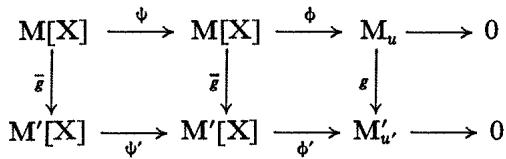
\includegraphics[keepaspectratio]{images/part004_f53e3a23.jpg}}

是交换的。

条件 \(g \circ u = u' \circ g\) 由 (43) 显然是使 \(g\) 成为 A{[}X{]}-同态的必要条件；它是充分的，因为它由归纳法蕴含 \(g \circ u^n = u'^n \circ g\) （对每个整数 \(n > 0\) ）。另一方面，对于所有 \(x \in M\) 以及所有 \(p \in A[X]\) ，

\[
\phi^ {\prime} (\bar {g} (p \otimes x)) = \phi^ {\prime} (p \otimes g (x)) = p (u ^ {\prime}) (g (x)) = g (p (u) (x)) = g (\phi (p \otimes x))
\]

和

\[
\bar {u} ^ {\prime} (\bar {g} (\boldsymbol {p} \otimes x)) = \bar {u} ^ {\prime} (\boldsymbol {p} \otimes g (x)) = \boldsymbol {p} \otimes u ^ {\prime} (g (x)) = \boldsymbol {p} \otimes g (u (x)) = \bar {g} (\bar {u} (\boldsymbol {p} \otimes x))
\]

这证明了图表(48)的交换性。

\subsection{自同态的特征多项式}

设 M 是维数为 n 的自由 A-模，u 是 M 的一个自同态。考虑两个不定元的多项式环 A{[}X, Y{]} 以及 A{[}X, Y{]}-模 M{[}X, Y{]} = A{[}X, Y{]} ⊗\_A M；令 \(\bar{u}\) 为由 u 典范地导出的 A{[}X, Y{]}-模 M{[}X, Y{]} 的自同态（II，§5，第1号）。由第 5 号命题 11 可知，

\[
\det (\mathbf {X} - \mathbf {Y} \bar {\boldsymbol {u}}) = \sum_ {j = 0} ^ {n} (- 1) ^ {j} \operatorname{Tr} \left(\bigwedge^ {j} (u)\right) \mathbf {X} ^ {n - j} \mathbf {Y} ^ {j}\tag{49}
\]

这是因为，若 \(U\) 是 \(u\) 关于某个基 \((e_i)_{1 \leqslant i \leqslant n}\) （ \(\mathbf{M}\) 的）的矩阵，则 \(U\) 就是 \(\bar{u}\) 关于基 \((1 \otimes e_i)_{1 \leqslant i \leqslant n}\) （ \(\mathbf{M}[\mathbf{X}, \mathbf{Y}]\) 的）的矩阵，因此

\[
\operatorname{Tr} \left(\bigwedge^ {j} (\bar {u})\right) = \operatorname{Tr} \left(\bigwedge^ {j} (u)\right).
\]

定义 3. 设 M 为有限维自由 A-模，u 为 M 的一个自同态。自同态 X - \(\bar{u}\) （自由 A{[}X{]}-模 M{[}X{]} 的）的行列式称为 u 的特征多项式，记作 \(\chi_u(X)\) 。

若 \(\mathbf{M}\) 的秩为 \(n\) ，则由 (49) 可知

\[
\chi_ {u} (\mathbf {X}) = \sum_ {j = 0} ^ {n} (- 1) ^ {j} \operatorname{Tr} \left(\bigwedge^ {j} (u)\right) \mathbf {X} ^ {n - j}\tag{50}
\]

因为 \(\operatorname{det}(\mathbf{X} - \mathbf{Y}\bar{u}) = \operatorname{det}(\mathbf{X}.I_n + \mathbf{Y}U)\) 且 \(\operatorname{det}(\mathbf{X} - \bar{u}) = \operatorname{det}(\mathbf{X}.I_n - U)\) 。由此可以看出 \(\chi_u(\mathbf{X})\) 是一个次数为 \(n\) 的首一多项式，其中 \(\mathbf{X}^{n-1}\) 的系数是 \(-\mathrm{Tr}(u)\) ，常数项是 \((-1)^n \operatorname{det}(u)\) 。

命题 20（”凯莱-哈密顿定理”）。对于有限维自由 A-模的每个自同态 \(u\) ，有 \(\chi_u(u) = 0\) 。

在命题 18（§ 3，第 10 号）的记号下，对于所有 \(x \in \mathbf{M}\) ， \(\chi_u(u)(x)\) 是在映射 \(\phi\) 下 \(\chi_u(\mathbf{X}) \otimes x\) 的像。但若 \(v\) 是 \(\mathbf{M}[\mathbf{X}]\) 的自同态、即 \(\mathbf{X} - \bar{u}\) 的余转置（第 6 号），那么

\[
\chi_ {u} (\mathbf {X}) \otimes x = \chi_ {u} (\mathbf {X}) (1 \otimes x) = (\mathbf {X} - \bar {u}) (v (1 \otimes x))
\]

且结论由第 10 号的命题 18 得出。

\section{范数与迹}

在本段中，K 表示一个交换环，A 是一个带单位的结合 K-代数。每个 A-模均假定具有通过将标量限制到 K 而得到的 K-模结构。
